\documentclass[12pt,a4paper]{article}

\usepackage[a4paper,width=160mm,top=25mm,bottom=25mm]{geometry}

\usepackage{fancyhdr}
\pagestyle{fancy}
\fancyhf{}
\fancyhead[EL]{\nouppercase\leftmark}
\fancyhead[OR]{\nouppercase\rightmark}
\fancyhead[ER,OL]{\thepage}

\usepackage{url}
\usepackage[hidelinks]{hyperref}

\renewcommand{\linethickness}{0.05em}
\usepackage[brazil]{babel}   
\usepackage{titlesec}
\newcommand{\sectionbreak}{\clearpage}


\title{Processando a Informação: um livro prático de programação independente de linguagem 
\\\large\vspace{2cm}
Rogério Perino de Oliveira Neves 
\\\vspace{5mm}
Francisco de Assis Zampirolli
\\\large\vspace{2cm}
EDUFABC
\\ \url{editora.ufabc.edu.br}
\\\Huge\vspace{3cm}
Notas de Aulas inspiradas no livro
\\\Large\vspace{1cm}
Utilizando a(s) Linguagem(ns) de Programação: 
\\\Huge\vspace{1cm}
C
\\\large\vspace{1cm}
Exemplos adaptados para Correção Automática no Moodle+VPL
\vspace{2cm}}
\author{Francisco de Assis Zampirolli\vspace{1cm}}


    \usepackage[breakable]{tcolorbox}
    \usepackage{parskip} % Stop auto-indenting (to mimic markdown behaviour)
    

    % Basic figure setup, for now with no caption control since it's done
    % automatically by Pandoc (which extracts ![](path) syntax from Markdown).
    \usepackage{graphicx}
    % Maintain compatibility with old templates. Remove in nbconvert 6.0
    \let\Oldincludegraphics\includegraphics
    % Ensure that by default, figures have no caption (until we provide a
    % proper Figure object with a Caption API and a way to capture that
    % in the conversion process - todo).
    \usepackage{caption}
    \DeclareCaptionFormat{nocaption}{}
    \captionsetup{format=nocaption,aboveskip=0pt,belowskip=0pt}

    \usepackage{float}
    \floatplacement{figure}{H} % forces figures to be placed at the correct location
    \usepackage{xcolor} % Allow colors to be defined
    \usepackage{enumerate} % Needed for markdown enumerations to work
    \usepackage{geometry} % Used to adjust the document margins
    \usepackage{amsmath} % Equations
    \usepackage{amssymb} % Equations
    \usepackage{textcomp} % defines textquotesingle
    % Hack from http://tex.stackexchange.com/a/47451/13684:
    \AtBeginDocument{%
        \def\PYZsq{\textquotesingle}% Upright quotes in Pygmentized code
    }
    \usepackage{upquote} % Upright quotes for verbatim code
    \usepackage{eurosym} % defines \euro

    \usepackage{iftex}
    \ifPDFTeX
        \usepackage[T1]{fontenc}
        \IfFileExists{alphabeta.sty}{
              \usepackage{alphabeta}
          }{
              \usepackage[mathletters]{ucs}
              \usepackage[utf8x]{inputenc}
          }
    \else
        \usepackage{fontspec}
        \usepackage{unicode-math}
    \fi

    \usepackage{fancyvrb} % verbatim replacement that allows latex
    \usepackage{grffile} % extends the file name processing of package graphics
                         % to support a larger range
    \makeatletter % fix for old versions of grffile with XeLaTeX
    \@ifpackagelater{grffile}{2019/11/01}
    {
      % Do nothing on new versions
    }
    {
      \def\Gread@@xetex#1{%
        \IfFileExists{"\Gin@base".bb}%
        {\Gread@eps{\Gin@base.bb}}%
        {\Gread@@xetex@aux#1}%
      }
    }
    \makeatother
    \usepackage[Export]{adjustbox} % Used to constrain images to a maximum size
    \adjustboxset{max size={0.9\linewidth}{0.9\paperheight}}

    % The hyperref package gives us a pdf with properly built
    % internal navigation ('pdf bookmarks' for the table of contents,
    % internal cross-reference links, web links for URLs, etc.)
    \usepackage{hyperref}
    % The default LaTeX title has an obnoxious amount of whitespace. By default,
    % titling removes some of it. It also provides customization options.
    \usepackage{titling}
    \usepackage{longtable} % longtable support required by pandoc >1.10
    \usepackage{booktabs}  % table support for pandoc > 1.12.2
    \usepackage{array}     % table support for pandoc >= 2.11.3
    \usepackage{calc}      % table minipage width calculation for pandoc >= 2.11.1
    \usepackage[inline]{enumitem} % IRkernel/repr support (it uses the enumerate* environment)
    \usepackage[normalem]{ulem} % ulem is needed to support strikethroughs (\sout)
                                % normalem makes italics be italics, not underlines
    \usepackage{mathrsfs}
    

    
    % Colors for the hyperref package
    \definecolor{urlcolor}{rgb}{0,.145,.698}
    \definecolor{linkcolor}{rgb}{.71,0.21,0.01}
    \definecolor{citecolor}{rgb}{.12,.54,.11}

    % ANSI colors
    \definecolor{ansi-black}{HTML}{3E424D}
    \definecolor{ansi-black-intense}{HTML}{282C36}
    \definecolor{ansi-red}{HTML}{E75C58}
    \definecolor{ansi-red-intense}{HTML}{B22B31}
    \definecolor{ansi-green}{HTML}{00A250}
    \definecolor{ansi-green-intense}{HTML}{007427}
    \definecolor{ansi-yellow}{HTML}{DDB62B}
    \definecolor{ansi-yellow-intense}{HTML}{B27D12}
    \definecolor{ansi-blue}{HTML}{208FFB}
    \definecolor{ansi-blue-intense}{HTML}{0065CA}
    \definecolor{ansi-magenta}{HTML}{D160C4}
    \definecolor{ansi-magenta-intense}{HTML}{A03196}
    \definecolor{ansi-cyan}{HTML}{60C6C8}
    \definecolor{ansi-cyan-intense}{HTML}{258F8F}
    \definecolor{ansi-white}{HTML}{C5C1B4}
    \definecolor{ansi-white-intense}{HTML}{A1A6B2}
    \definecolor{ansi-default-inverse-fg}{HTML}{FFFFFF}
    \definecolor{ansi-default-inverse-bg}{HTML}{000000}

    % common color for the border for error outputs.
    \definecolor{outerrorbackground}{HTML}{FFDFDF}

    % commands and environments needed by pandoc snippets
    % extracted from the output of `pandoc -s`
    \providecommand{\tightlist}{%
      \setlength{\itemsep}{0pt}\setlength{\parskip}{0pt}}
    \DefineVerbatimEnvironment{Highlighting}{Verbatim}{commandchars=\\\{\}}
    % Add ',fontsize=\small' for more characters per line
    \newenvironment{Shaded}{}{}
    \newcommand{\KeywordTok}[1]{\textcolor[rgb]{0.00,0.44,0.13}{\textbf{{#1}}}}
    \newcommand{\DataTypeTok}[1]{\textcolor[rgb]{0.56,0.13,0.00}{{#1}}}
    \newcommand{\DecValTok}[1]{\textcolor[rgb]{0.25,0.63,0.44}{{#1}}}
    \newcommand{\BaseNTok}[1]{\textcolor[rgb]{0.25,0.63,0.44}{{#1}}}
    \newcommand{\FloatTok}[1]{\textcolor[rgb]{0.25,0.63,0.44}{{#1}}}
    \newcommand{\CharTok}[1]{\textcolor[rgb]{0.25,0.44,0.63}{{#1}}}
    \newcommand{\StringTok}[1]{\textcolor[rgb]{0.25,0.44,0.63}{{#1}}}
    \newcommand{\CommentTok}[1]{\textcolor[rgb]{0.38,0.63,0.69}{\textit{{#1}}}}
    \newcommand{\OtherTok}[1]{\textcolor[rgb]{0.00,0.44,0.13}{{#1}}}
    \newcommand{\AlertTok}[1]{\textcolor[rgb]{1.00,0.00,0.00}{\textbf{{#1}}}}
    \newcommand{\FunctionTok}[1]{\textcolor[rgb]{0.02,0.16,0.49}{{#1}}}
    \newcommand{\RegionMarkerTok}[1]{{#1}}
    \newcommand{\ErrorTok}[1]{\textcolor[rgb]{1.00,0.00,0.00}{\textbf{{#1}}}}
    \newcommand{\NormalTok}[1]{{#1}}

    % Additional commands for more recent versions of Pandoc
    \newcommand{\ConstantTok}[1]{\textcolor[rgb]{0.53,0.00,0.00}{{#1}}}
    \newcommand{\SpecialCharTok}[1]{\textcolor[rgb]{0.25,0.44,0.63}{{#1}}}
    \newcommand{\VerbatimStringTok}[1]{\textcolor[rgb]{0.25,0.44,0.63}{{#1}}}
    \newcommand{\SpecialStringTok}[1]{\textcolor[rgb]{0.73,0.40,0.53}{{#1}}}
    \newcommand{\ImportTok}[1]{{#1}}
    \newcommand{\DocumentationTok}[1]{\textcolor[rgb]{0.73,0.13,0.13}{\textit{{#1}}}}
    \newcommand{\AnnotationTok}[1]{\textcolor[rgb]{0.38,0.63,0.69}{\textbf{\textit{{#1}}}}}
    \newcommand{\CommentVarTok}[1]{\textcolor[rgb]{0.38,0.63,0.69}{\textbf{\textit{{#1}}}}}
    \newcommand{\VariableTok}[1]{\textcolor[rgb]{0.10,0.09,0.49}{{#1}}}
    \newcommand{\ControlFlowTok}[1]{\textcolor[rgb]{0.00,0.44,0.13}{\textbf{{#1}}}}
    \newcommand{\OperatorTok}[1]{\textcolor[rgb]{0.40,0.40,0.40}{{#1}}}
    \newcommand{\BuiltInTok}[1]{{#1}}
    \newcommand{\ExtensionTok}[1]{{#1}}
    \newcommand{\PreprocessorTok}[1]{\textcolor[rgb]{0.74,0.48,0.00}{{#1}}}
    \newcommand{\AttributeTok}[1]{\textcolor[rgb]{0.49,0.56,0.16}{{#1}}}
    \newcommand{\InformationTok}[1]{\textcolor[rgb]{0.38,0.63,0.69}{\textbf{\textit{{#1}}}}}
    \newcommand{\WarningTok}[1]{\textcolor[rgb]{0.38,0.63,0.69}{\textbf{\textit{{#1}}}}}


    % Define a nice break command that doesn't care if a line doesn't already
    % exist.
    \def\br{\hspace*{\fill} \\* }
    % Math Jax compatibility definitions
    \def\gt{>}
    \def\lt{<}
    \let\Oldtex\TeX
    \let\Oldlatex\LaTeX
    \renewcommand{\TeX}{\textrm{\Oldtex}}
    \renewcommand{\LaTeX}{\textrm{\Oldlatex}}
    % Document parameters
    % Document title
    %\title{cap1.part1.c}
    
    
    
    
    
% Pygments definitions
\makeatletter
\def\PY@reset{\let\PY@it=\relax \let\PY@bf=\relax%
    \let\PY@ul=\relax \let\PY@tc=\relax%
    \let\PY@bc=\relax \let\PY@ff=\relax}
\def\PY@tok#1{\csname PY@tok@#1\endcsname}
\def\PY@toks#1+{\ifx\relax#1\empty\else%
    \PY@tok{#1}\expandafter\PY@toks\fi}
\def\PY@do#1{\PY@bc{\PY@tc{\PY@ul{%
    \PY@it{\PY@bf{\PY@ff{#1}}}}}}}
\def\PY#1#2{\PY@reset\PY@toks#1+\relax+\PY@do{#2}}

\@namedef{PY@tok@w}{\def\PY@tc##1{\textcolor[rgb]{0.73,0.73,0.73}{##1}}}
\@namedef{PY@tok@c}{\let\PY@it=\textit\def\PY@tc##1{\textcolor[rgb]{0.24,0.48,0.48}{##1}}}
\@namedef{PY@tok@cp}{\def\PY@tc##1{\textcolor[rgb]{0.61,0.40,0.00}{##1}}}
\@namedef{PY@tok@k}{\let\PY@bf=\textbf\def\PY@tc##1{\textcolor[rgb]{0.00,0.50,0.00}{##1}}}
\@namedef{PY@tok@kp}{\def\PY@tc##1{\textcolor[rgb]{0.00,0.50,0.00}{##1}}}
\@namedef{PY@tok@kt}{\def\PY@tc##1{\textcolor[rgb]{0.69,0.00,0.25}{##1}}}
\@namedef{PY@tok@o}{\def\PY@tc##1{\textcolor[rgb]{0.40,0.40,0.40}{##1}}}
\@namedef{PY@tok@ow}{\let\PY@bf=\textbf\def\PY@tc##1{\textcolor[rgb]{0.67,0.13,1.00}{##1}}}
\@namedef{PY@tok@nb}{\def\PY@tc##1{\textcolor[rgb]{0.00,0.50,0.00}{##1}}}
\@namedef{PY@tok@nf}{\def\PY@tc##1{\textcolor[rgb]{0.00,0.00,1.00}{##1}}}
\@namedef{PY@tok@nc}{\let\PY@bf=\textbf\def\PY@tc##1{\textcolor[rgb]{0.00,0.00,1.00}{##1}}}
\@namedef{PY@tok@nn}{\let\PY@bf=\textbf\def\PY@tc##1{\textcolor[rgb]{0.00,0.00,1.00}{##1}}}
\@namedef{PY@tok@ne}{\let\PY@bf=\textbf\def\PY@tc##1{\textcolor[rgb]{0.80,0.25,0.22}{##1}}}
\@namedef{PY@tok@nv}{\def\PY@tc##1{\textcolor[rgb]{0.10,0.09,0.49}{##1}}}
\@namedef{PY@tok@no}{\def\PY@tc##1{\textcolor[rgb]{0.53,0.00,0.00}{##1}}}
\@namedef{PY@tok@nl}{\def\PY@tc##1{\textcolor[rgb]{0.46,0.46,0.00}{##1}}}
\@namedef{PY@tok@ni}{\let\PY@bf=\textbf\def\PY@tc##1{\textcolor[rgb]{0.44,0.44,0.44}{##1}}}
\@namedef{PY@tok@na}{\def\PY@tc##1{\textcolor[rgb]{0.41,0.47,0.13}{##1}}}
\@namedef{PY@tok@nt}{\let\PY@bf=\textbf\def\PY@tc##1{\textcolor[rgb]{0.00,0.50,0.00}{##1}}}
\@namedef{PY@tok@nd}{\def\PY@tc##1{\textcolor[rgb]{0.67,0.13,1.00}{##1}}}
\@namedef{PY@tok@s}{\def\PY@tc##1{\textcolor[rgb]{0.73,0.13,0.13}{##1}}}
\@namedef{PY@tok@sd}{\let\PY@it=\textit\def\PY@tc##1{\textcolor[rgb]{0.73,0.13,0.13}{##1}}}
\@namedef{PY@tok@si}{\let\PY@bf=\textbf\def\PY@tc##1{\textcolor[rgb]{0.64,0.35,0.47}{##1}}}
\@namedef{PY@tok@se}{\let\PY@bf=\textbf\def\PY@tc##1{\textcolor[rgb]{0.67,0.36,0.12}{##1}}}
\@namedef{PY@tok@sr}{\def\PY@tc##1{\textcolor[rgb]{0.64,0.35,0.47}{##1}}}
\@namedef{PY@tok@ss}{\def\PY@tc##1{\textcolor[rgb]{0.10,0.09,0.49}{##1}}}
\@namedef{PY@tok@sx}{\def\PY@tc##1{\textcolor[rgb]{0.00,0.50,0.00}{##1}}}
\@namedef{PY@tok@m}{\def\PY@tc##1{\textcolor[rgb]{0.40,0.40,0.40}{##1}}}
\@namedef{PY@tok@gh}{\let\PY@bf=\textbf\def\PY@tc##1{\textcolor[rgb]{0.00,0.00,0.50}{##1}}}
\@namedef{PY@tok@gu}{\let\PY@bf=\textbf\def\PY@tc##1{\textcolor[rgb]{0.50,0.00,0.50}{##1}}}
\@namedef{PY@tok@gd}{\def\PY@tc##1{\textcolor[rgb]{0.63,0.00,0.00}{##1}}}
\@namedef{PY@tok@gi}{\def\PY@tc##1{\textcolor[rgb]{0.00,0.52,0.00}{##1}}}
\@namedef{PY@tok@gr}{\def\PY@tc##1{\textcolor[rgb]{0.89,0.00,0.00}{##1}}}
\@namedef{PY@tok@ge}{\let\PY@it=\textit}
\@namedef{PY@tok@gs}{\let\PY@bf=\textbf}
\@namedef{PY@tok@gp}{\let\PY@bf=\textbf\def\PY@tc##1{\textcolor[rgb]{0.00,0.00,0.50}{##1}}}
\@namedef{PY@tok@go}{\def\PY@tc##1{\textcolor[rgb]{0.44,0.44,0.44}{##1}}}
\@namedef{PY@tok@gt}{\def\PY@tc##1{\textcolor[rgb]{0.00,0.27,0.87}{##1}}}
\@namedef{PY@tok@err}{\def\PY@bc##1{{\setlength{\fboxsep}{\string -\fboxrule}\fcolorbox[rgb]{1.00,0.00,0.00}{1,1,1}{\strut ##1}}}}
\@namedef{PY@tok@kc}{\let\PY@bf=\textbf\def\PY@tc##1{\textcolor[rgb]{0.00,0.50,0.00}{##1}}}
\@namedef{PY@tok@kd}{\let\PY@bf=\textbf\def\PY@tc##1{\textcolor[rgb]{0.00,0.50,0.00}{##1}}}
\@namedef{PY@tok@kn}{\let\PY@bf=\textbf\def\PY@tc##1{\textcolor[rgb]{0.00,0.50,0.00}{##1}}}
\@namedef{PY@tok@kr}{\let\PY@bf=\textbf\def\PY@tc##1{\textcolor[rgb]{0.00,0.50,0.00}{##1}}}
\@namedef{PY@tok@bp}{\def\PY@tc##1{\textcolor[rgb]{0.00,0.50,0.00}{##1}}}
\@namedef{PY@tok@fm}{\def\PY@tc##1{\textcolor[rgb]{0.00,0.00,1.00}{##1}}}
\@namedef{PY@tok@vc}{\def\PY@tc##1{\textcolor[rgb]{0.10,0.09,0.49}{##1}}}
\@namedef{PY@tok@vg}{\def\PY@tc##1{\textcolor[rgb]{0.10,0.09,0.49}{##1}}}
\@namedef{PY@tok@vi}{\def\PY@tc##1{\textcolor[rgb]{0.10,0.09,0.49}{##1}}}
\@namedef{PY@tok@vm}{\def\PY@tc##1{\textcolor[rgb]{0.10,0.09,0.49}{##1}}}
\@namedef{PY@tok@sa}{\def\PY@tc##1{\textcolor[rgb]{0.73,0.13,0.13}{##1}}}
\@namedef{PY@tok@sb}{\def\PY@tc##1{\textcolor[rgb]{0.73,0.13,0.13}{##1}}}
\@namedef{PY@tok@sc}{\def\PY@tc##1{\textcolor[rgb]{0.73,0.13,0.13}{##1}}}
\@namedef{PY@tok@dl}{\def\PY@tc##1{\textcolor[rgb]{0.73,0.13,0.13}{##1}}}
\@namedef{PY@tok@s2}{\def\PY@tc##1{\textcolor[rgb]{0.73,0.13,0.13}{##1}}}
\@namedef{PY@tok@sh}{\def\PY@tc##1{\textcolor[rgb]{0.73,0.13,0.13}{##1}}}
\@namedef{PY@tok@s1}{\def\PY@tc##1{\textcolor[rgb]{0.73,0.13,0.13}{##1}}}
\@namedef{PY@tok@mb}{\def\PY@tc##1{\textcolor[rgb]{0.40,0.40,0.40}{##1}}}
\@namedef{PY@tok@mf}{\def\PY@tc##1{\textcolor[rgb]{0.40,0.40,0.40}{##1}}}
\@namedef{PY@tok@mh}{\def\PY@tc##1{\textcolor[rgb]{0.40,0.40,0.40}{##1}}}
\@namedef{PY@tok@mi}{\def\PY@tc##1{\textcolor[rgb]{0.40,0.40,0.40}{##1}}}
\@namedef{PY@tok@il}{\def\PY@tc##1{\textcolor[rgb]{0.40,0.40,0.40}{##1}}}
\@namedef{PY@tok@mo}{\def\PY@tc##1{\textcolor[rgb]{0.40,0.40,0.40}{##1}}}
\@namedef{PY@tok@ch}{\let\PY@it=\textit\def\PY@tc##1{\textcolor[rgb]{0.24,0.48,0.48}{##1}}}
\@namedef{PY@tok@cm}{\let\PY@it=\textit\def\PY@tc##1{\textcolor[rgb]{0.24,0.48,0.48}{##1}}}
\@namedef{PY@tok@cpf}{\let\PY@it=\textit\def\PY@tc##1{\textcolor[rgb]{0.24,0.48,0.48}{##1}}}
\@namedef{PY@tok@c1}{\let\PY@it=\textit\def\PY@tc##1{\textcolor[rgb]{0.24,0.48,0.48}{##1}}}
\@namedef{PY@tok@cs}{\let\PY@it=\textit\def\PY@tc##1{\textcolor[rgb]{0.24,0.48,0.48}{##1}}}

\def\PYZbs{\char`\\}
\def\PYZus{\char`\_}
\def\PYZob{\char`\{}
\def\PYZcb{\char`\}}
\def\PYZca{\char`\^}
\def\PYZam{\char`\&}
\def\PYZlt{\char`\<}
\def\PYZgt{\char`\>}
\def\PYZsh{\char`\#}
\def\PYZpc{\char`\%}
\def\PYZdl{\char`\$}
\def\PYZhy{\char`\-}
\def\PYZsq{\char`\'}
\def\PYZdq{\char`\"}
\def\PYZti{\char`\~}
% for compatibility with earlier versions
\def\PYZat{@}
\def\PYZlb{[}
\def\PYZrb{]}
\makeatother


    % For linebreaks inside Verbatim environment from package fancyvrb.
    \makeatletter
        \newbox\Wrappedcontinuationbox
        \newbox\Wrappedvisiblespacebox
        \newcommand*\Wrappedvisiblespace {\textcolor{red}{\textvisiblespace}}
        \newcommand*\Wrappedcontinuationsymbol {\textcolor{red}{\llap{\tiny$\m@th\hookrightarrow$}}}
        \newcommand*\Wrappedcontinuationindent {3ex }
        \newcommand*\Wrappedafterbreak {\kern\Wrappedcontinuationindent\copy\Wrappedcontinuationbox}
        % Take advantage of the already applied Pygments mark-up to insert
        % potential linebreaks for TeX processing.
        %        {, <, #, %, $, ' and ": go to next line.
        %        _, }, ^, &, >, - and ~: stay at end of broken line.
        % Use of \textquotesingle for straight quote.
        \newcommand*\Wrappedbreaksatspecials {%
            \def\PYGZus{\discretionary{\char`\_}{\Wrappedafterbreak}{\char`\_}}%
            \def\PYGZob{\discretionary{}{\Wrappedafterbreak\char`\{}{\char`\{}}%
            \def\PYGZcb{\discretionary{\char`\}}{\Wrappedafterbreak}{\char`\}}}%
            \def\PYGZca{\discretionary{\char`\^}{\Wrappedafterbreak}{\char`\^}}%
            \def\PYGZam{\discretionary{\char`\&}{\Wrappedafterbreak}{\char`\&}}%
            \def\PYGZlt{\discretionary{}{\Wrappedafterbreak\char`\<}{\char`\<}}%
            \def\PYGZgt{\discretionary{\char`\>}{\Wrappedafterbreak}{\char`\>}}%
            \def\PYGZsh{\discretionary{}{\Wrappedafterbreak\char`\#}{\char`\#}}%
            \def\PYGZpc{\discretionary{}{\Wrappedafterbreak\char`\%}{\char`\%}}%
            \def\PYGZdl{\discretionary{}{\Wrappedafterbreak\char`\$}{\char`\$}}%
            \def\PYGZhy{\discretionary{\char`\-}{\Wrappedafterbreak}{\char`\-}}%
            \def\PYGZsq{\discretionary{}{\Wrappedafterbreak\textquotesingle}{\textquotesingle}}%
            \def\PYGZdq{\discretionary{}{\Wrappedafterbreak\char`\"}{\char`\"}}%
            \def\PYGZti{\discretionary{\char`\~}{\Wrappedafterbreak}{\char`\~}}%
        }
        % Some characters . , ; ? ! / are not pygmentized.
        % This macro makes them "active" and they will insert potential linebreaks
        \newcommand*\Wrappedbreaksatpunct {%
            \lccode`\~`\.\lowercase{\def~}{\discretionary{\hbox{\char`\.}}{\Wrappedafterbreak}{\hbox{\char`\.}}}%
            \lccode`\~`\,\lowercase{\def~}{\discretionary{\hbox{\char`\,}}{\Wrappedafterbreak}{\hbox{\char`\,}}}%
            \lccode`\~`\;\lowercase{\def~}{\discretionary{\hbox{\char`\;}}{\Wrappedafterbreak}{\hbox{\char`\;}}}%
            \lccode`\~`\:\lowercase{\def~}{\discretionary{\hbox{\char`\:}}{\Wrappedafterbreak}{\hbox{\char`\:}}}%
            \lccode`\~`\?\lowercase{\def~}{\discretionary{\hbox{\char`\?}}{\Wrappedafterbreak}{\hbox{\char`\?}}}%
            \lccode`\~`\!\lowercase{\def~}{\discretionary{\hbox{\char`\!}}{\Wrappedafterbreak}{\hbox{\char`\!}}}%
            \lccode`\~`\/\lowercase{\def~}{\discretionary{\hbox{\char`\/}}{\Wrappedafterbreak}{\hbox{\char`\/}}}%
            \catcode`\.\active
            \catcode`\,\active
            \catcode`\;\active
            \catcode`\:\active
            \catcode`\?\active
            \catcode`\!\active
            \catcode`\/\active
            \lccode`\~`\~
        }
    \makeatother

    \let\OriginalVerbatim=\Verbatim
    \makeatletter
    \renewcommand{\Verbatim}[1][1]{%
        %\parskip\z@skip
        \sbox\Wrappedcontinuationbox {\Wrappedcontinuationsymbol}%
        \sbox\Wrappedvisiblespacebox {\FV@SetupFont\Wrappedvisiblespace}%
        \def\FancyVerbFormatLine ##1{\hsize\linewidth
            \vtop{\raggedright\hyphenpenalty\z@\exhyphenpenalty\z@
                \doublehyphendemerits\z@\finalhyphendemerits\z@
                \strut ##1\strut}%
        }%
        % If the linebreak is at a space, the latter will be displayed as visible
        % space at end of first line, and a continuation symbol starts next line.
        % Stretch/shrink are however usually zero for typewriter font.
        \def\FV@Space {%
            \nobreak\hskip\z@ plus\fontdimen3\font minus\fontdimen4\font
            \discretionary{\copy\Wrappedvisiblespacebox}{\Wrappedafterbreak}
            {\kern\fontdimen2\font}%
        }%

        % Allow breaks at special characters using \PYG... macros.
        \Wrappedbreaksatspecials
        % Breaks at punctuation characters . , ; ? ! and / need catcode=\active
        \OriginalVerbatim[#1,codes*=\Wrappedbreaksatpunct]%
    }
    \makeatother

    % Exact colors from NB
    \definecolor{incolor}{HTML}{303F9F}
    \definecolor{outcolor}{HTML}{D84315}
    \definecolor{cellborder}{HTML}{CFCFCF}
    \definecolor{cellbackground}{HTML}{F7F7F7}

    % prompt
    \makeatletter
    \newcommand{\boxspacing}{\kern\kvtcb@left@rule\kern\kvtcb@boxsep}
    \makeatother
    \newcommand{\prompt}[4]{
        {\ttfamily\llap{{\color{#2}[#3]:\hspace{3pt}#4}}\vspace{-\baselineskip}}
    }
    

    
    % Prevent overflowing lines due to hard-to-break entities
    \sloppy
    % Setup hyperref package
    \hypersetup{
      breaklinks=true,  % so long urls are correctly broken across lines
      colorlinks=true,
      urlcolor=urlcolor,
      linkcolor=linkcolor,
      citecolor=citecolor,
      }
    % Slightly bigger margins than the latex defaults
    
    \geometry{verbose,tmargin=1in,bmargin=1in,lmargin=1in,rmargin=1in}
    
    

\begin{document}
    
    
\clearpage\maketitle
\thispagestyle{empty}
\tableofcontents

    
    

    
    \hypertarget{processando-a-informauxe7uxe3o-cap.-1-fundamentos}{%
\section{Processando a Informação: Cap. 1:
Fundamentos}\label{processando-a-informauxe7uxe3o-cap.-1-fundamentos}}

    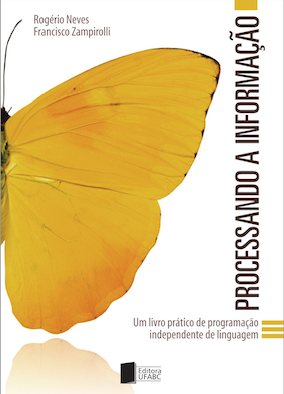
\includegraphics{"figs/Capa_Processando_Informacao.jpg"}

Este caderno (Notebook) é parte complementar \emph{online} do livro
\textbf{\href{https://editora.ufabc.edu.br/matematica-e-ciencias-da-computacao/58-processando-a-informacao}{Processando
a Informação}: um livro prático de programação independente de
linguagem}, que deve ser consultado no caso de dúvidas sobre os temas
apresentados.

\begin{quote}
Este conteúdo pode ser copiado e alterado livremente e foi inspirado
nesse livro.
\end{quote}

    \textbf{Bem vindo ao Google Colab!}

Se você é novo no uso do Colab, assista os vários
\href{https://www.youtube.com/results?search_query=introdu\%C3\%A7\%C3\%A3o+ao+colab}{vídeos
em português} explicando a plataforma. Existem também \textbf{workbooks}
introdutórios para o uso do Python e do Colab na
\href{https://colab.research.google.com/}{página principal} do projeto.

De forma muito resumida, o Colab combina \textbf{células de texto e de
código}. Esse paradigma de juntar documentação e código em um único
documento foi introduzido por Donald Knuth em 1984
{[}\href{https://www-cs-faculty.stanford.edu/~knuth/}{ref1},
\href{http://www.literateprogramming.com}{ref2}{]}.

    \hypertarget{instruuxe7uxf5es}{%
\subsection{Instruções}\label{instruuxe7uxf5es}}

    \begin{itemize}
\tightlist
\item
  É recomendado tirar uma cópia deste notebook clicando em
  \textbf{``Arquivo''}--\textgreater{}\textbf{``Salvar cópia no
  drive''}. Desta forma você poderá editá-lo e executar os campos de
  código sempre que quiser, sem perder os seu progresso ao fechar esta
  página. Essa cópia estará disponível na pasta \textbf{Colab
  Notebooks}, no seu Google Drive.
\item
  Para poder editar uma \textbf{CÉLULA DE TEXTO} (como esta), basta dar
  dois cliques na célula e editar, que pode ser visualizada na aba à
  direita (ou abaixo), ou pressionar Shift+Enter, ou ainda clicando em
  outra célula.
\item
  No Colab também tem a \textbf{CÉLULA DE CÓDIGO}, que pode ser
  executada com essa combinação de teclas, ou clique no botão
  \textbf{``executar''} ou \textbf{``play''} para ver a saída do código
  entrado.
\item
  É recomendado seguir a ordem sugerida dos exercícios, uma vez que
  familiaridade com os conceitos introduzidos são esperados nos
  exercícios seguintes.
\item
  É possível rodar códigos independentes em IDEs e também \emph{online},
  utilizando navegadores, como o Chrome: https://ideone.com/,
  https://www.codechef.com/ide, https://replit.com/,
  https://www.jdoodle.com
\item
  É possível também rodar códigos no seu celular, utilizando navegadores
  acessando esses links.
\item
  Esse arquivo com extensão \texttt{ipynb} pode ser editado também no
  Jupyter Notebook - https://jupyter.org.
\end{itemize}

    \hypertarget{sumuxe1rio}{%
\subsection{Sumário}\label{sumuxe1rio}}

\begin{itemize}
\tightlist
\item
  Introdução à arquitetura de computadores; Hardware e Software
\item
  Algoritmos, fluxogramas e lógica de programação
\item
  Conceitos de linguagens de programação
\item
  Variáveis, tipos de dados e organização da memória
\item
  Operadores e precedência
\item
  Aprendendo a programar
\item
  Revisão deste capítulo
\item
  Exercícios
\end{itemize}

    \hypertarget{introduuxe7uxe3o-uxe0-arquitetura-de-computadores}{%
\subsection{Introdução à Arquitetura de
Computadores}\label{introduuxe7uxe3o-uxe0-arquitetura-de-computadores}}

    A arquitetura (ou organização dos principais componentes) mais conhecida
de computadores foi introduzida por John Von Newmann, em 1936, ver
Figura abaixo.

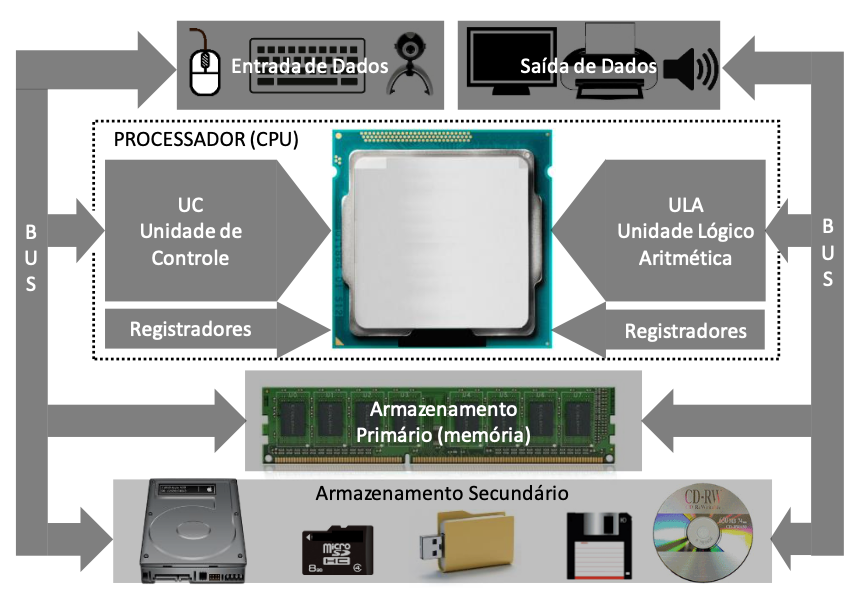
\includegraphics{"figs/image02.png"}

    \begin{figure}
\centering
\caption{Captura de Tela 2021-03-26 às 11.26.59.png}
\end{figure}

    \begin{itemize}
\item
  Um software é um conjunto de linhas de código, armazenado em arquivo
  na memória secundária ou na RAM, que pode ser execudado, instrução por
  instrução na CPU.
\item
  Essas linhas de código são instruções que o computador consegue
  executar, mas que podem ter sido traduzidas de um \textbf{Algoritmo}.
\end{itemize}

    \hypertarget{algoritmos-fluxogramas-e-luxf3gica-de-programauxe7uxe3o}{%
\subsection{Algoritmos, Fluxogramas e Lógica de
Programação}\label{algoritmos-fluxogramas-e-luxf3gica-de-programauxe7uxe3o}}

    \begin{verbatim}
ALGORITMO (algumas definições):
1. Um processo ou conjunto de regras a serem seguidas em cálculo ou outra
operação de solução de problemas, especialmente por um computador.
2. Processo de resolução de um problema constituído por uma sequência 
ordenada e bem definida de passos que, em tempo finito, conduzem à 
solução do problema ou indicam que, para o mesmo, não existem soluções.
\end{verbatim}

    Um exemplo de algoritmo: solução de uma equação do segundo grau no
formato \(ax^2 + bx + c\), dados \(a\), \(b\) e \(c\):

\begin{enumerate}
\def\labelenumi{\arabic{enumi}.}
\tightlist
\item
  Calcule \(\Delta\) com a fórmula \(\Delta = b^2-4ac\);
\item
  Se \(\Delta < 0\), \(x\) não possui raízes reais;
\item
  Se \(\Delta = 0\), \(x\) possui duas raízes reais idênticas;
\item
  Se \(\Delta > 0\), \(x\) possui duas raízes reais e distintas;
\item
  Calcule \(x\) usando a equação.
\end{enumerate}

    \hypertarget{pseudocuxf3digo}{%
\subsubsection{Pseudocódigo}\label{pseudocuxf3digo}}

    \begin{itemize}
\item
  Essa sequência de passos definidas no algoritmo anterior, se incluída
  as instruções \texttt{leia(algo)} e \texttt{escreva(algo)}, poder ser
  definida como um \textbf{pseudocódigo}.
\item
  Esse \textbf{pseudocódigo} é para humanos conseguirem entender os
  passos de um algoritmo, de uma forma ``mais próxima'' de como os
  computadores processam as instruções, utilizando uma linguagem de
  programação, definidas na próxima seção.
\end{itemize}

Veja a seguir um exemplo de pseudocódigo do algoritmo anterior:

    \begin{verbatim}
leia(a,b,c)
calcular delta = b**2-4*a*c
se delta < 0: 
   escreva(x não possui raízes reais)
   fim do programa
se delta = 0:
   escreva(x possui duas raízes reais idênticas)
se delta > 0:
   escreva(x possui duas raízes reais e distintas)
calcule x=a*x*x+b*x+c
escreva(x)
\end{verbatim}

    Observe que em um pseudocódigo existe uma descrição um pouco mais
detalhada das instruções, que em um algoritmo, mas não é uma descrição
muito rígida/formal, como existem nas linguagems de programação.

    \hypertarget{fluxogramas}{%
\subsubsection{Fluxogramas}\label{fluxogramas}}

    \begin{itemize}
\item
  Os algoritmos, além de poderem ser representados por listas de
  instruções, como no último exemplo, podem ser representados
  graficamente para facilitar seu entendimento.
\item
  Os fluxogramas e diagramas de atividades da UML (\emph{Unified
  Modelling Language}) estão entre as representações mais usadas.
\item
  Ambos, bem similares, usam formas e setas para indicar operações e
  seus fluxos.
\item
  A Figura abaixo ilustra um exemplo de fluxograma.
\end{itemize}

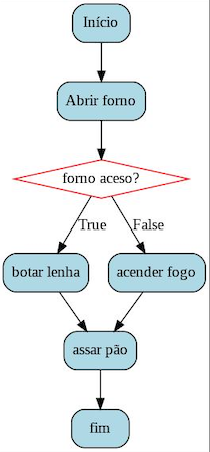
\includegraphics{"figs/flowchart.jpg"}

    \begin{figure}
\centering
\caption{flowchart.jpg}
\end{figure}

    Esse fluxograma foi gerado automaticamente rodando as duas células de
código abaixo.

\textbf{Observação:} apesar do livro texto ser independente de
linguangem, alguns códigos nesta adaptação em Colab serão apresentados
na linguagem de programação Python, pela facilidade didática na
apresentação de conteúdos. Assim, os detalhes desses códigos não serão
apresentados, pois foge o escopo.

    \begin{tcolorbox}[breakable, size=fbox, boxrule=1pt, pad at break*=1mm,colback=cellbackground, colframe=cellborder]
\prompt{In}{incolor}{ }{\boxspacing}
\begin{Verbatim}[commandchars=\\\{\}]
\PY{c+c1}{\PYZsh{} instalando algumas bibliotecas no servidor do Colab (Linux)}
\PY{o}{!}apt\PYZhy{}get install graphviz libgraphviz\PYZhy{}dev pkg\PYZhy{}config
\PY{o}{!}pip install txtoflow
\end{Verbatim}
\end{tcolorbox}

    \begin{tcolorbox}[breakable, size=fbox, boxrule=1pt, pad at break*=1mm,colback=cellbackground, colframe=cellborder]
\prompt{In}{incolor}{ }{\boxspacing}
\begin{Verbatim}[commandchars=\\\{\}]
\PY{c+c1}{\PYZsh{} importando a biblioteca txtflow para gerar fluxograma a partir de código}
\PY{k+kn}{from} \PY{n+nn}{txtoflow} \PY{k+kn}{import} \PY{n}{txtoflow}

\PY{c+c1}{\PYZsh{} definindo o pseudocódigo e passando como entrada de dados para gerar o fluxograma}
\PY{n}{txtoflow}\PY{o}{.}\PY{n}{generate}\PY{p}{(}
    \PY{l+s+sd}{\PYZsq{}\PYZsq{}\PYZsq{}}
\PY{l+s+sd}{    Início;}
\PY{l+s+sd}{    Abrir forno;}
\PY{l+s+sd}{    if (forno aceso?) \PYZob{}}
\PY{l+s+sd}{        botar lenha;}
\PY{l+s+sd}{    \PYZcb{} else \PYZob{}}
\PY{l+s+sd}{        acender fogo;}
\PY{l+s+sd}{    \PYZcb{}}
\PY{l+s+sd}{    assar pão;}
\PY{l+s+sd}{    fim;}
\PY{l+s+sd}{    \PYZsq{}\PYZsq{}\PYZsq{}}
\PY{p}{)}
\end{Verbatim}
\end{tcolorbox}

    \begin{itemize}
\tightlist
\item
  Após rodar a célula de código acima, ver o arquivo
  \texttt{flowchart.jpg} clicando no ícone de pasta à esquerda.
\end{itemize}

    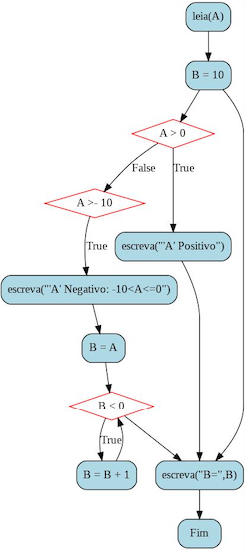
\includegraphics{"figs/flowchart2.jpg"}

\begin{itemize}
\tightlist
\item
  Veja um outro fluxograma gerado a partir da célula abaixo;
  \textgreater{} Apesar deste primeiro fluxograma ser intuitivo, os
  detalhes (principalmente do próximo fluxograma) serão vistos durantes
  este curso!
\end{itemize}

    \begin{tcolorbox}[breakable, size=fbox, boxrule=1pt, pad at break*=1mm,colback=cellbackground, colframe=cellborder]
\prompt{In}{incolor}{ }{\boxspacing}
\begin{Verbatim}[commandchars=\\\{\}]
\PY{c+c1}{\PYZsh{} definindo uma variável do tipo texto (string) para armazenar o pseudocódigo}
\PY{n}{alg2} \PY{o}{=} \PY{l+s+s1}{\PYZsq{}\PYZsq{}\PYZsq{}}
\PY{l+s+s1}{leia(A);}
\PY{l+s+s1}{B = 10;}
\PY{l+s+s1}{if ( A \PYZgt{} 0 ) }\PY{l+s+s1}{\PYZob{}}
\PY{l+s+s1}{  escreva(}\PY{l+s+s1}{\PYZdq{}}\PY{l+s+s1}{\PYZsq{}}\PY{l+s+s1}{A}\PY{l+s+s1}{\PYZsq{}}\PY{l+s+s1}{ Positivo}\PY{l+s+s1}{\PYZdq{}}\PY{l+s+s1}{);}
\PY{l+s+s1}{\PYZcb{} else if ( A \PYZgt{}\PYZhy{} 10 ) }\PY{l+s+s1}{\PYZob{}}
\PY{l+s+s1}{  escreva(}\PY{l+s+s1}{\PYZdq{}}\PY{l+s+s1}{\PYZsq{}}\PY{l+s+s1}{A}\PY{l+s+s1}{\PYZsq{}}\PY{l+s+s1}{ Negativo: \PYZhy{}10\PYZlt{}A\PYZlt{}=0}\PY{l+s+s1}{\PYZdq{}}\PY{l+s+s1}{);}
\PY{l+s+s1}{  B = A;}
\PY{l+s+s1}{  while ( B \PYZlt{} 0 ) }\PY{l+s+s1}{\PYZob{}}
\PY{l+s+s1}{    B = B + 1;}
\PY{l+s+s1}{  \PYZcb{}}
\PY{l+s+s1}{\PYZcb{}}
\PY{l+s+s1}{escreva(}\PY{l+s+s1}{\PYZdq{}}\PY{l+s+s1}{B=}\PY{l+s+s1}{\PYZdq{}}\PY{l+s+s1}{,B);}
\PY{l+s+s1}{Fim;}\PY{l+s+s1}{\PYZsq{}\PYZsq{}\PYZsq{}}

\PY{c+c1}{\PYZsh{} criando o fluxograma}
\PY{n}{txtoflow}\PY{o}{.}\PY{n}{generate}\PY{p}{(}\PY{n}{alg2}\PY{p}{)}
\end{Verbatim}
\end{tcolorbox}

    \begin{figure}
\centering
\caption{flowchart2.jpg}
\end{figure}

    \begin{itemize}
\tightlist
\item
  Qual o valor final de B neste algoritmo, se o valor lido foi
  \texttt{A=-5}?
\item
  Experimente também essa ferramenta \emph{online}:
  \href{https://app.code2flow.com/}{code2flow}
\end{itemize}

    \hypertarget{fluxograma-a-partir-de-cuxf3digo-python}{%
\paragraph{Fluxograma a partir de código
python}\label{fluxograma-a-partir-de-cuxf3digo-python}}

    A sequência de códigos a seguir geram fluxogramas na própria célula de
código, diferente de salvar em arquivo de imagem. Além disso, a entrada
é um código em python, diferente do exemplo anterior que está em
pseudocódigo.

    \begin{tcolorbox}[breakable, size=fbox, boxrule=1pt, pad at break*=1mm,colback=cellbackground, colframe=cellborder]
\prompt{In}{incolor}{ }{\boxspacing}
\begin{Verbatim}[commandchars=\\\{\}]
\PY{o}{!}pip install \PYZhy{}\PYZhy{}upgrade git+https://github.com/innovationOUtside/flowchart\PYZus{}js\PYZus{}jp\PYZus{}proxy\PYZus{}widget.git
\end{Verbatim}
\end{tcolorbox}

    \begin{tcolorbox}[breakable, size=fbox, boxrule=1pt, pad at break*=1mm,colback=cellbackground, colframe=cellborder]
\prompt{In}{incolor}{ }{\boxspacing}
\begin{Verbatim}[commandchars=\\\{\}]
\PY{k+kn}{from} \PY{n+nn}{google}\PY{n+nn}{.}\PY{n+nn}{colab} \PY{k+kn}{import} \PY{n}{output}
\PY{n}{output}\PY{o}{.}\PY{n}{enable\PYZus{}custom\PYZus{}widget\PYZus{}manager}\PY{p}{(}\PY{p}{)}
\end{Verbatim}
\end{tcolorbox}

    \begin{tcolorbox}[breakable, size=fbox, boxrule=1pt, pad at break*=1mm,colback=cellbackground, colframe=cellborder]
\prompt{In}{incolor}{ }{\boxspacing}
\begin{Verbatim}[commandchars=\\\{\}]
\PY{n}{alg3} \PY{o}{=} \PY{l+s+s1}{\PYZsq{}\PYZsq{}\PYZsq{}}
\PY{l+s+s1}{A = int(input())}
\PY{l+s+s1}{B = 10}
\PY{l+s+s1}{if A \PYZgt{} 0:}
\PY{l+s+s1}{  print(}\PY{l+s+s1}{\PYZdq{}}\PY{l+s+s1}{\PYZsq{}}\PY{l+s+s1}{A}\PY{l+s+s1}{\PYZsq{}}\PY{l+s+s1}{ Positivo}\PY{l+s+s1}{\PYZdq{}}\PY{l+s+s1}{)}
\PY{l+s+s1}{elif A \PYZgt{} \PYZhy{}10:}
\PY{l+s+s1}{  print(}\PY{l+s+s1}{\PYZdq{}}\PY{l+s+s1}{\PYZsq{}}\PY{l+s+s1}{A}\PY{l+s+s1}{\PYZsq{}}\PY{l+s+s1}{ Negativo: \PYZhy{}10\PYZlt{}A\PYZlt{}=0}\PY{l+s+s1}{\PYZdq{}}\PY{l+s+s1}{)}
\PY{l+s+s1}{  B = A}
\PY{l+s+s1}{  while B \PYZlt{} 0:}
\PY{l+s+s1}{    B = B + 1}
\PY{l+s+s1}{    print(B)}
\PY{l+s+s1}{print(}\PY{l+s+s1}{\PYZdq{}}\PY{l+s+s1}{B=}\PY{l+s+s1}{\PYZdq{}}\PY{l+s+s1}{,B)}\PY{l+s+s1}{\PYZsq{}\PYZsq{}\PYZsq{}}
\end{Verbatim}
\end{tcolorbox}

    \begin{tcolorbox}[breakable, size=fbox, boxrule=1pt, pad at break*=1mm,colback=cellbackground, colframe=cellborder]
\prompt{In}{incolor}{ }{\boxspacing}
\begin{Verbatim}[commandchars=\\\{\}]
\PY{k+kn}{from} \PY{n+nn}{pyflowchart} \PY{k+kn}{import} \PY{n}{Flowchart}
\PY{n}{fc} \PY{o}{=} \PY{n}{Flowchart}\PY{o}{.}\PY{n}{from\PYZus{}code}\PY{p}{(}\PY{n}{alg3}\PY{p}{)}
\PY{n}{flowchart} \PY{o}{=} \PY{n}{fc}\PY{o}{.}\PY{n}{flowchart}\PY{p}{(}\PY{p}{)}
\end{Verbatim}
\end{tcolorbox}

    \begin{tcolorbox}[breakable, size=fbox, boxrule=1pt, pad at break*=1mm,colback=cellbackground, colframe=cellborder]
\prompt{In}{incolor}{ }{\boxspacing}
\begin{Verbatim}[commandchars=\\\{\}]
\PY{k+kn}{from} \PY{n+nn}{jp\PYZus{}flowchartjs}\PY{n+nn}{.}\PY{n+nn}{jp\PYZus{}flowchartjs} \PY{k+kn}{import} \PY{n}{FlowchartWidget}

\PY{n}{testEmbed} \PY{o}{=} \PY{n}{FlowchartWidget}\PY{p}{(}\PY{p}{)}
\PY{n}{testEmbed}\PY{o}{.}\PY{n}{charter}\PY{p}{(}\PY{n}{flowchart}\PY{p}{)}
\PY{n}{testEmbed}
\end{Verbatim}
\end{tcolorbox}

    \begin{itemize}
\item
  Comparando os dois fluxogramas anteriores é possível notar que é mais
  difícil ler esse último por falta de cor e por ter cruzamentos entre
  retas.
\item
  Achou alguma ferramenta mais interessante para gerar fluxograma neste
  Colab? Compartilhe!

  \begin{itemize}
  \tightlist
  \item
    Por exemplo, seria interessante criar um fluxograma a partir de uma
    célula de código, contendo várias instruções, e não a partir de um
    texto, como ocorre na ferramenta \emph{online} anterior.
  \end{itemize}
\end{itemize}

    \hypertarget{conceitos-de-linguagens-de-programauxe7uxe3o}{%
\subsection{Conceitos de Linguagens de
Programação}\label{conceitos-de-linguagens-de-programauxe7uxe3o}}

    Linguagem é um conjunto de regras usado para se definir uma forma de
comunicação. São conceitos fundamentais de qualquer linguagem, não só em
computação:

\begin{itemize}
\tightlist
\item
  \textbf{sintaxe:} o arranjo de palavras e sua disposição em um
  discurso para criar frases bem formadas e relacionadas de forma lógica
  em uma linguagem;
\item
  \textbf{semântica:} o ramo da linguística preocupado com a lógica e o
  significado das palavras. sub-ramos incluem a semântica formal e a
  semântica lexical.
\end{itemize}

    \hypertarget{nuxedveis-de-liguagens}{%
\subsubsection{Níveis de Liguagens}\label{nuxedveis-de-liguagens}}

    Nível de linguagem diz respeito à proximidade em que ela se encontra da
linguagem natural humana.

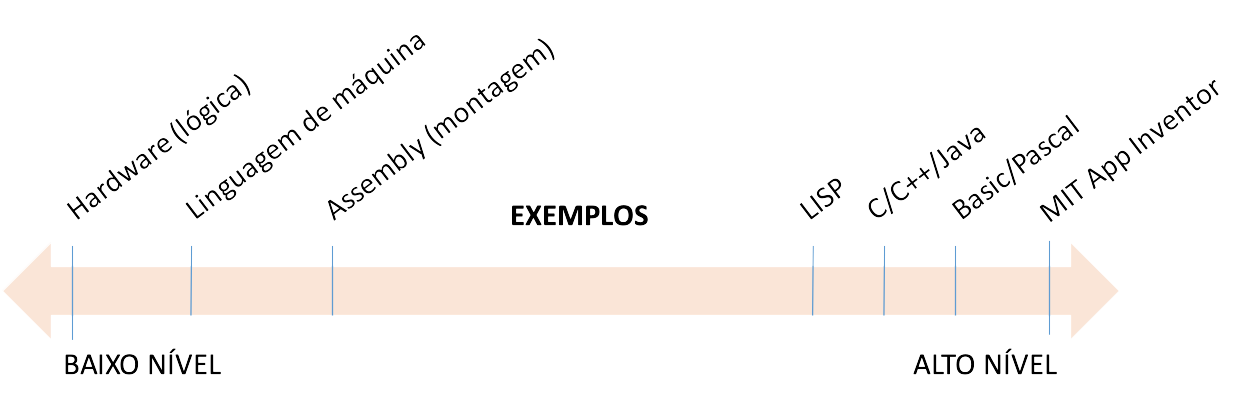
\includegraphics{"figs/image03.png"}

    \begin{figure}
\centering
\caption{image.png}
\end{figure}

    \hypertarget{linguagem-compilada-vs-interpretada}{%
\subsubsection{Linguagem Compilada vs
Interpretada}\label{linguagem-compilada-vs-interpretada}}

    \begin{itemize}
\item
  A \textbf{compilação} é o nome dado ao processo de traduzir um código
  escrito em uma linguagem de mais alto-nível para código de máquina,
  que poderá ser executado na arquitetura apropriada para o qual foi
  compilado.

  \begin{itemize}
  \tightlist
  \item
    Exemplos de linguagens compiladas: C, CPP (ou C++), Pascal e
    Fortran.
  \end{itemize}
\item
  Em \textbf{linguagens interpretadas}, os comandos do programa são
  transformados em código nativo durante a sua execução, geralmente por
  um outro programa, necessário para seu funcionamento.

  \begin{itemize}
  \tightlist
  \item
    Exemplos de linguagens interpretadas: python (nesse Colab), R,
    matlab.
  \end{itemize}
\item
  A exceção é a linguagem \textbf{Java}, que compila um código binário
  em bytes (\textbf{bytecode}), para ser executado não em uma
  arquitetura real específica, mas sim pela \textbf{máquina virtual
  Java} (JVM), que é um \textbf{programa nativo} (isto é, é necessário
  um JVM compilado para cada arquitetura) responsável por transformar
  \emph{bytecode} na linguagem de máquina nativa do processador em tempo
  de execução (\textbf{runtime}).
\item
  A existência de JVM para a maioria das plataformas aumentou em muito a
  portabilidade dos programas. A \textbf{portabilidade} foi uma das
  principais motivações para a criação da linguagem Java.
\end{itemize}

    \hypertarget{estruturas-de-cuxf3digo}{%
\subsubsection{Estruturas de Código}\label{estruturas-de-cuxf3digo}}

    Independente da linguagem escolhida, as estruturas fundamentais de
código que estarão presentes em todas elas são:

\begin{enumerate}
\def\labelenumi{\arabic{enumi}.}
\tightlist
\item
  \textbf{Código sequencial:} os comandos são executados na ordem em que
  aparecem;
\item
  \textbf{Módulos de código (funções ou métodos):} conjuntos de comandos
  agrupados em sub-rotinas ou subprogramas;
\item
  \textbf{Desvios condicionais:} dada uma condição, existem dois
  caminhos possíveis (duas linhas) de execução;
\item
  \textbf{Estruturas de repetição ou laços:} conjuntos de comandos que
  se repetem enquanto uma dada condição for satisfeita.
\end{enumerate}

    \hypertarget{deburauxe7uxe3o-de-cuxf3digo-debug}{%
\subsubsection{Deburação de Código
(DEBUG)}\label{deburauxe7uxe3o-de-cuxf3digo-debug}}

    \begin{itemize}
\item
  É referido como depuração ou ``debugação'' o árduo processo de busca e
  correção dos erros de programação no código escrito em linguagens de
  programação.
\item
  Ferramentas de depuração são de grande valia para auxiliar na busca e
  correção destes erros.
\item
  Alguns dos erros comuns encontrados em código, do menos grave ao mais
  sério, são:
\end{itemize}

    \begin{quote}
\begin{enumerate}
\def\labelenumi{\arabic{enumi}.}
\tightlist
\item
  \textbf{Erro de semântica:} palavras reservadas ou operações escritas
  de forma errada;
\item
  \textbf{Erro de sintaxe:} envolve o uso inapropriado do formato dos
  comandos;
\item
  \textbf{Erro de organização:} blocos de código, aspas ou uso de
  parênteses inconsistentes -- ocorre quando se abre um bloco de código
  ou de operadores (com chaves, colchetes ou parênteses) ou um campo de
  texto (com aspas) sem fechar ou se fecha sem abrir;
\item
  \textbf{Erro de lógica:} também conhecido como \emph{Cerberus} (o cão
  de guarda do inferno), ocorre quando os comandos estão sintaticamente
  corretos, na semântica correta, e escritos consistentemente, porém em
  ordem, forma ou disposição que produz um resultado diferente do
  desejado. Resultado este que, frequentemente, causa travamento da
  execução do programa ou até mesmo do computador.
\end{enumerate}
\end{quote}

    \hypertarget{ambientes-de-desenvolvimento-integrados}{%
\subsubsection{Ambientes de Desenvolvimento
Integrados}\label{ambientes-de-desenvolvimento-integrados}}

    Ambientes de desenvolvimento integrado ou IDE (\emph{Integrated
Developing Environment}), como são conhecidos, oferecem uma combinação
de ferramentas úteis para escrita, execução e depuração do código de
programas.

    Algumas ferramentas de desenvolvimento populares do tipo IDE são: -
\textbf{Eclipse} (C, CPP, Java, PHP, android, etc); - \textbf{NetBeans}
(C, CPP, Java, ruby, HTMl5, PHP, etc); - \textbf{PyCharm} (Python,
JavaScript, CoffeeScript, XML, HTML/XHTML); - \textbf{Xcode} (IDE de
desenvolvimento para dispositivos Apple); - \textbf{Visual studio} (C,
CPP, C\#, visual Basic, entre outros, voltado para o desenvolvimento de
programas na plataforma Windows). -
\textbf{\href{https://vscode.dev}{VSCODE}} (versão \emph{online} de
código aberto do \emph{Visual studio}. Para download e uso local:
https://code.visualstudio.com/download).

    Mais alguns links úteis para programar em várias linguagens
\emph{online}:

\begin{itemize}
\item
  https://colab.research.google.com
\item
  https://replit.com/languages
\item
  http://www.drjava.org
\item
  https://sourceforge.net/projects/nbportable
\item
  https://ideone.com
\item
  https://www.codechef.com/ide

  Python:
\item
  https://www.programiz.com/python-programming/online-compiler/
\item
  https://www.onlinegdb.com/online\_python\_compiler
\item
  https://www.tutorialspoint.com/execute\_python\_online.php
\item
  https://www.python.org/shell/
\item
  http://pythontutor.com
\end{itemize}

Ou para Baixar IDE's: * https://www.anaconda.com/distribution *
https://netbeans.org

Mais links interessantes: * https://learnxinyminutes.com/docs/python3 *
https://learnxinyminutes.com/docs/java *
https://learnxinyminutes.com/docs/c * https://youtu.be/UNSoPa-XQN0

Tem outros links interessantes que não estão nestas listas? Compartilhe!

    \hypertarget{algumas-estatuxedsticas-sobre-linguagens-mais-usadas}{%
\paragraph{Algumas Estatísticas sobre Linguagens Mais
Usadas:}\label{algumas-estatuxedsticas-sobre-linguagens-mais-usadas}}

\begin{itemize}
\tightlist
\item
  https://insights.stackoverflow.com/trends?tags=python\%2Cjava\%2Cjavascript\\
\item
  \href{https://profdanielbrandao.wordpress.com/2019/03/01/o-incrivel-crescimento-da-linguagem-python/}{reportagem}
\item
  https://insights.stackoverflow.com/survey/2020
\item
  https://insights.stackoverflow.com/survey/2020\#most-popular-technologies
\end{itemize}

    \hypertarget{variuxe1veis}{%
\subsection{Variáveis}\label{variuxe1veis}}

    \begin{itemize}
\tightlist
\item
  Uma variável em programação de computadores é um indicador ou
  `apelido' (\emph{alias}) atribuído a um endereço de memória que contém
  um dado guardado.
\item
  Os elementos na memória, representados por variáveis, podem conter
  apenas um ou múltiplos valores, e são codificados na memória de acordo
  com o tipo específico do dado, com formato e número de bits apropriado
  para mantê-los.
\end{itemize}

    \hypertarget{uso-de-variuxe1veis}{%
\subsubsection{Uso de Variáveis}\label{uso-de-variuxe1veis}}

    Em qualquer linguagem, um valor pode ser atribuído a uma variável
através do operador de atribuição, por exemplo: ``\texttt{=}''.

    \hypertarget{exemplos-de-variuxe1veis-do-tipo-inteiro}{%
\paragraph{Exemplos de variáveis do tipo
inteiro:}\label{exemplos-de-variuxe1veis-do-tipo-inteiro}}

    \begin{itemize}
\item
  As próximas células de código em Python podem ser executadas clicando
  em \texttt{{[}\ {]}} ou seta de \emph{play}, na margem esquerda.
\item
  Se o seu objetivo é aprender outras linguagens de programação, essas
  células em Python podem ser utilizadas como comparativos.
\end{itemize}

    \begin{tcolorbox}[breakable, size=fbox, boxrule=1pt, pad at break*=1mm,colback=cellbackground, colframe=cellborder]
\prompt{In}{incolor}{ }{\boxspacing}
\begin{Verbatim}[commandchars=\\\{\}]
\PY{n}{idade} \PY{o}{=} \PY{l+m+mi}{20}\PY{p}{;}     \PY{c+c1}{\PYZsh{} esse é um comentário}
\PY{n}{anoAtual} \PY{o}{=} \PY{l+m+mi}{2021} \PY{c+c1}{\PYZsh{} observer que \PYZsq{};\PYZsq{} é opcional em python e javascript}
\end{Verbatim}
\end{tcolorbox}

    A leitura correta para o código representado acima é \textbf{``a
variável \texttt{idade} recebe o valor 20''}.

    \begin{tcolorbox}[breakable, size=fbox, boxrule=1pt, pad at break*=1mm,colback=cellbackground, colframe=cellborder]
\prompt{In}{incolor}{ }{\boxspacing}
\begin{Verbatim}[commandchars=\\\{\}]
\PY{n}{idade}
\end{Verbatim}
\end{tcolorbox}

    \begin{tcolorbox}[breakable, size=fbox, boxrule=1pt, pad at break*=1mm,colback=cellbackground, colframe=cellborder]
\prompt{In}{incolor}{ }{\boxspacing}
\begin{Verbatim}[commandchars=\\\{\}]
\PY{n}{anoNascimento} \PY{o}{=} \PY{n}{anoAtual} \PY{o}{\PYZhy{}} \PY{n}{idade}
\PY{n}{anoNascimento}
\end{Verbatim}
\end{tcolorbox}

    \hypertarget{exemplo-de-variuxe1vel-do-tipo-texto-string}{%
\paragraph{\texorpdfstring{Exemplo de variável do tipo texto
(\emph{string})}{Exemplo de variável do tipo texto (string)}}\label{exemplo-de-variuxe1vel-do-tipo-texto-string}}

    \begin{tcolorbox}[breakable, size=fbox, boxrule=1pt, pad at break*=1mm,colback=cellbackground, colframe=cellborder]
\prompt{In}{incolor}{ }{\boxspacing}
\begin{Verbatim}[commandchars=\\\{\}]
\PY{n}{nomeAluno} \PY{o}{=} \PY{l+s+s1}{\PYZsq{}}\PY{l+s+s1}{Rafael Morais}\PY{l+s+s1}{\PYZsq{}}
\PY{n}{nomeAluno}
\end{Verbatim}
\end{tcolorbox}

    \begin{tcolorbox}[breakable, size=fbox, boxrule=1pt, pad at break*=1mm,colback=cellbackground, colframe=cellborder]
\prompt{In}{incolor}{ }{\boxspacing}
\begin{Verbatim}[commandchars=\\\{\}]
\PY{n}{nomeAluno} \PY{o}{=} \PY{l+s+s2}{\PYZdq{}}\PY{l+s+s2}{Rafael Morais}\PY{l+s+s2}{\PYZdq{}}
\PY{n}{nomeAluno}
\end{Verbatim}
\end{tcolorbox}

    Observe que o texto deve ficar entre aspas simples ou duplas (dependendo
das linguagem escolhida).

    \hypertarget{exemplo-de-variuxe1vel-do-tipo-real}{%
\paragraph{Exemplo de variável do tipo
real}\label{exemplo-de-variuxe1vel-do-tipo-real}}

    \begin{tcolorbox}[breakable, size=fbox, boxrule=1pt, pad at break*=1mm,colback=cellbackground, colframe=cellborder]
\prompt{In}{incolor}{ }{\boxspacing}
\begin{Verbatim}[commandchars=\\\{\}]
\PY{n}{pi} \PY{o}{=} \PY{l+m+mf}{3.1415926535897932}
\PY{n}{pi}
\end{Verbatim}
\end{tcolorbox}

    Observe que tem que usar `.' para separar as casas decimais.

    \hypertarget{nomenclatura}{%
\paragraph{Nomenclatura}\label{nomenclatura}}

    \begin{itemize}
\item
  Os nomes das variáveis podem conter letras, números e alguns
  caracteres especiais, desde que não sejam empregados pelo lexema da
  linguagem (símbolos dos operadores matemáticos, lógicos e relacionais,
  por exemplo).
\item
  Em geral, o nome da variável deve começar por uma letra ou, dependendo
  da linguagem, algum caractere especial.
\item
  Como regra geral os nomes de variáveis não devem começar com números
  ou conter espaços.
\end{itemize}

    Exemplos de variáveis válidas e inválidas:

\begin{longtable}[]{@{}ll@{}}
\toprule
Válido & Inválido\tabularnewline
\midrule
\endhead
idade4 & 4idade\tabularnewline
Nome\_Completo & Nome Completo\tabularnewline
resta\_um & resta-um\tabularnewline
V8S9F0D7S7D9 & V@R!V\&+\tabularnewline
\bottomrule
\end{longtable}

    \hypertarget{operadores-e-preceduxeancia}{%
\subsection{Operadores e
precedência}\label{operadores-e-preceduxeancia}}

    As linguagens reservam alguns caracteres para uso em operadores ou
indicadores de tipo.

    \hypertarget{operadores-aritmeticos}{%
\subsubsection{Operadores aritmeticos}\label{operadores-aritmeticos}}

    **

Tabela: Operadores aritméticos em Java/C/CPP/JS

**

\begin{longtable}[]{@{}ll@{}}
\toprule
operador & descrição\tabularnewline
\midrule
\endhead
+ & soma com\tabularnewline
- & subtração por\tabularnewline
* & multiplicação por\tabularnewline
/ & divisão por\tabularnewline
\% & resto da divisão por\tabularnewline
++ & incremento\tabularnewline
-- & decremento\tabularnewline
\bottomrule
\end{longtable}

    \hypertarget{operadores-relacionais}{%
\subsubsection{Operadores relacionais}\label{operadores-relacionais}}

    **

Tabela: Operadores relacionais em Java/C/CPP/JS

**

\begin{longtable}[]{@{}ll@{}}
\toprule
operador & descrição\tabularnewline
\midrule
\endhead
== & é igual a\tabularnewline
!= & é diferente de\tabularnewline
\textgreater{} & é maior que\tabularnewline
\textless{} & é menor que\tabularnewline
\textgreater= & é maior ou igual a\tabularnewline
\textless= & é menor ou igual a\tabularnewline
\bottomrule
\end{longtable}

    \hypertarget{operadores-luxf3gicos}{%
\subsubsection{Operadores lógicos}\label{operadores-luxf3gicos}}

    **

Tabela: Operadores lógicos binários em Java/C/CPP/JS

**

\begin{longtable}[]{@{}ll@{}}
\toprule
operador & descrição\tabularnewline
\midrule
\endhead
x \textbf{\&\&} y & True se ambos também forem\tabularnewline
x \textbf{\&} y & True se ambos também forem bit-a-bit\tabularnewline
x \textbf{\textbar\textbar{}} y & False se ambos também
forem\tabularnewline
x \textbf{\textbar{}} y & False se ambos também forem
bit-a-bit\tabularnewline
\textbf{!} x & contrário de x\tabularnewline
\textbf{\textasciitilde{}} x & contrário de x bit-a-bit\tabularnewline
\textbf{\^{}} x & ou exclusivo \texttt{XOR} bit-a-bit\tabularnewline
\textbf{\textless\textless{}}N & \emph{shift-left}, adiciona N zeros à
direita do número binário\tabularnewline
\textbf{\textless\textless{}}N & \emph{shift-right}, elimina N zeros à
direita do número binário\tabularnewline
\bottomrule
\end{longtable}

    \hypertarget{operadores-de-atribuiuxe7uxe3o}{%
\subsubsection{Operadores de
atribuição}\label{operadores-de-atribuiuxe7uxe3o}}

    **

Tabela: Operadores de atribuição em Python/Java/C/CPP/JS

**

\begin{longtable}[]{@{}ll@{}}
\toprule
operador & descrição\tabularnewline
\midrule
\endhead
= & recebe o valor de\tabularnewline
+= & é somado ao valor de\tabularnewline
-= & é subtraído do valor de\tabularnewline
*= & é multiplicado pelo valor de\tabularnewline
/= & é dividido pelo valor de\tabularnewline
\%= & recebe o resto da divisão por\tabularnewline
similarmente & \textgreater\textgreater=, \textless\textless=,
\&=,\tabularnewline
\bottomrule
\end{longtable}

    \begin{center}\rule{0.5\linewidth}{0.5pt}\end{center}

    \hypertarget{preceduxeancia-de-operadores}{%
\subsubsection{Precedência de
Operadores}\label{preceduxeancia-de-operadores}}

    Quando utilizados em uma expressão, os operadores apresentados
anteriormente são executados em ordem de precedência, de forma
semelhante como fazemos em equações matemáticas, com somas, subtrações,
multiplicações, divisões, exponenciais, etc. (testar Tabela abaixo na
linguagem escolhida).

    **

Tabela: Precedência de Operadores

**

\begin{longtable}[]{@{}lll@{}}
\toprule
\begin{minipage}[b]{0.26\columnwidth}\raggedright
Categoria\strut
\end{minipage} & \begin{minipage}[b]{0.44\columnwidth}\raggedright
Operador\strut
\end{minipage} & \begin{minipage}[b]{0.21\columnwidth}\raggedright
Associatividade\strut
\end{minipage}\tabularnewline
\midrule
\endhead
\begin{minipage}[t]{0.26\columnwidth}\raggedright
Pós-fixado\strut
\end{minipage} & \begin{minipage}[t]{0.44\columnwidth}\raggedright
() (parênteses, operador ponto)\strut
\end{minipage} & \begin{minipage}[t]{0.21\columnwidth}\raggedright
\(\rightarrow\) Esquerda para a direita\strut
\end{minipage}\tabularnewline
\begin{minipage}[t]{0.26\columnwidth}\raggedright
Índice\strut
\end{minipage} & \begin{minipage}[t]{0.44\columnwidth}\raggedright
{[}{]}\strut
\end{minipage} & \begin{minipage}[t]{0.21\columnwidth}\raggedright
\(\rightarrow\) Esquerda para a direita\strut
\end{minipage}\tabularnewline
\begin{minipage}[t]{0.26\columnwidth}\raggedright
Unário\strut
\end{minipage} & \begin{minipage}[t]{0.44\columnwidth}\raggedright
++ - - ! \textasciitilde{} (incremento, decremento)\strut
\end{minipage} & \begin{minipage}[t]{0.21\columnwidth}\raggedright
\(\leftarrow\) Direita para a esquerda\strut
\end{minipage}\tabularnewline
\begin{minipage}[t]{0.26\columnwidth}\raggedright
Multiplicativo\strut
\end{minipage} & \begin{minipage}[t]{0.44\columnwidth}\raggedright
* / \% (vezes, dividido, resto)\strut
\end{minipage} & \begin{minipage}[t]{0.21\columnwidth}\raggedright
\(\rightarrow\) Esquerda para a direita\strut
\end{minipage}\tabularnewline
\begin{minipage}[t]{0.26\columnwidth}\raggedright
Aditivo\strut
\end{minipage} & \begin{minipage}[t]{0.44\columnwidth}\raggedright
+ - (soma, subtração)\strut
\end{minipage} & \begin{minipage}[t]{0.21\columnwidth}\raggedright
\(\rightarrow\) Esquerda para a direita\strut
\end{minipage}\tabularnewline
\begin{minipage}[t]{0.26\columnwidth}\raggedright
Shift binário\strut
\end{minipage} & \begin{minipage}[t]{0.44\columnwidth}\raggedright
\textgreater\textgreater{} \textgreater\textgreater\textgreater{}
\textless\textless{}\strut
\end{minipage} & \begin{minipage}[t]{0.21\columnwidth}\raggedright
\(\rightarrow\) Esquerda para a direita\strut
\end{minipage}\tabularnewline
\begin{minipage}[t]{0.26\columnwidth}\raggedright
Relacional\strut
\end{minipage} & \begin{minipage}[t]{0.44\columnwidth}\raggedright
\textgreater{} \textgreater= \textless{} \textless=\strut
\end{minipage} & \begin{minipage}[t]{0.21\columnwidth}\raggedright
\(\rightarrow\) Esquerda para a direita\strut
\end{minipage}\tabularnewline
\begin{minipage}[t]{0.26\columnwidth}\raggedright
Igualdade\strut
\end{minipage} & \begin{minipage}[t]{0.44\columnwidth}\raggedright
== != (é igual a, é diferente de)\strut
\end{minipage} & \begin{minipage}[t]{0.21\columnwidth}\raggedright
\(\rightarrow\) Esquerda para a direita\strut
\end{minipage}\tabularnewline
\begin{minipage}[t]{0.26\columnwidth}\raggedright
E (AND) bit-a-bit\strut
\end{minipage} & \begin{minipage}[t]{0.44\columnwidth}\raggedright
\&\strut
\end{minipage} & \begin{minipage}[t]{0.21\columnwidth}\raggedright
\(\rightarrow\) Esquerda para a direita\strut
\end{minipage}\tabularnewline
\begin{minipage}[t]{0.26\columnwidth}\raggedright
XOR bit-a-bit\strut
\end{minipage} & \begin{minipage}[t]{0.44\columnwidth}\raggedright
\^{}\strut
\end{minipage} & \begin{minipage}[t]{0.21\columnwidth}\raggedright
\(\rightarrow\) Esquerda para a direita\strut
\end{minipage}\tabularnewline
\begin{minipage}[t]{0.26\columnwidth}\raggedright
Ou (OR) bit-a-bit\strut
\end{minipage} & \begin{minipage}[t]{0.44\columnwidth}\raggedright
\textbar{}\strut
\end{minipage} & \begin{minipage}[t]{0.21\columnwidth}\raggedright
\(\rightarrow\) Esquerda para a direita\strut
\end{minipage}\tabularnewline
\begin{minipage}[t]{0.26\columnwidth}\raggedright
E lógico\strut
\end{minipage} & \begin{minipage}[t]{0.44\columnwidth}\raggedright
\&\&\strut
\end{minipage} & \begin{minipage}[t]{0.21\columnwidth}\raggedright
\(\rightarrow\) Esquerda para a direita\strut
\end{minipage}\tabularnewline
\begin{minipage}[t]{0.26\columnwidth}\raggedright
Ou lógico\strut
\end{minipage} & \begin{minipage}[t]{0.44\columnwidth}\raggedright
\textbar\textbar{}\strut
\end{minipage} & \begin{minipage}[t]{0.21\columnwidth}\raggedright
\(\rightarrow\) Esquerda para a direita\strut
\end{minipage}\tabularnewline
\begin{minipage}[t]{0.26\columnwidth}\raggedright
Condicional\strut
\end{minipage} & \begin{minipage}[t]{0.44\columnwidth}\raggedright
?:\strut
\end{minipage} & \begin{minipage}[t]{0.21\columnwidth}\raggedright
\(\leftarrow\) Direita para a esquerda\strut
\end{minipage}\tabularnewline
\begin{minipage}[t]{0.26\columnwidth}\raggedright
Atribuição\strut
\end{minipage} & \begin{minipage}[t]{0.44\columnwidth}\raggedright
= += -= *= /= \%= \textgreater\textgreater= \textless\textless= \&=
\^{}= \textbar=\strut
\end{minipage} & \begin{minipage}[t]{0.21\columnwidth}\raggedright
\(\leftarrow\) Direita para a esquerda\strut
\end{minipage}\tabularnewline
\bottomrule
\end{longtable}

    \hypertarget{tipos-buxe1sicos-de-variuxe1veis}{%
\paragraph{Tipos básicos de
variáveis}\label{tipos-buxe1sicos-de-variuxe1veis}}

    \hypertarget{conversuxf5es-de-tipos-de-variuxe1veis}{%
\paragraph{Conversões de tipos de
variáveis}\label{conversuxf5es-de-tipos-de-variuxe1veis}}

    **

Tabela: Tipos de variáveis em Java/C/CPP/JS

**

\begin{longtable}[]{@{}lllll@{}}
\toprule
\endhead
\textbf{Tipo} & \textbf{Descrição} & \textbf{n.~Bits} & \textbf{Mínimo}
& \textbf{Máximo ( valor )}\tabularnewline
& & & &\tabularnewline
\textbf{Tipos inteiros+sinal} & & & &\tabularnewline
byte & inteiro de 1 byte & \(8\) & \(-128\) & \(127\)\tabularnewline
short & inteiro curto & \(16\) & \(-2^{15}\) &
\(2^{15}-1\)\tabularnewline
int & inteiro & \(32\) & \(-2^{31}\) & \(2^{31}-1\)\tabularnewline
long & inteiro longo & \(64\) & \(-2^{63}\) &
\(2^{63}-1\)\tabularnewline
& & & &\tabularnewline
\textbf{Tipos reais+ponto flut.} & & & &\tabularnewline
float & precisão simples & \(32\) & \(2^{-149}\) &
\((2-2^{-23})2^{127}\)\tabularnewline
double & precisão dupla & \(64\) & \(2^{-1074}\) &
\((2-2^{-52}))2^{1023}\)\tabularnewline
& & & &\tabularnewline
\textbf{Tipos lógicos} & & & &\tabularnewline
boolean & valor booleano & \(1\) & \(false\) & \(true\)\tabularnewline
& & & &\tabularnewline
\textbf{Tipos alfanuméricos} & & & &\tabularnewline
char & caractere unicode & \(16\) & \(0\) & \(2^{16}-1\)\tabularnewline
& & & &\tabularnewline
\textbf{Classecadeia de caract.} & & & &\tabularnewline
String & sequência n chars & \(16*n\) & - & -\tabularnewline
& & & &\tabularnewline
\textbf{Outras} & & & &\tabularnewline
void & variável vazia & \(0\) & - & -\tabularnewline
\bottomrule
\end{longtable}

    **

Tabela: Exemplos de conversão de valores entre tipos de variáveis

**

\begin{longtable}[]{@{}lll@{}}
\toprule
\endhead
\begin{minipage}[t]{0.21\columnwidth}\raggedright
\textbf{Conversão}\strut
\end{minipage} & \begin{minipage}[t]{0.22\columnwidth}\raggedright
\textbf{Método}\strut
\end{minipage} & \begin{minipage}[t]{0.48\columnwidth}\raggedright
\textbf{Exemplo}\strut
\end{minipage}\tabularnewline
\begin{minipage}[t]{0.21\columnwidth}\raggedright
\strut
\end{minipage} & \begin{minipage}[t]{0.22\columnwidth}\raggedright
\strut
\end{minipage} & \begin{minipage}[t]{0.48\columnwidth}\raggedright
\strut
\end{minipage}\tabularnewline
\begin{minipage}[t]{0.21\columnwidth}\raggedright
\strut
\end{minipage} & \begin{minipage}[t]{0.22\columnwidth}\raggedright
\strut
\end{minipage} & \begin{minipage}[t]{0.48\columnwidth}\raggedright
\textbf{C/C++/Java}\strut
\end{minipage}\tabularnewline
\begin{minipage}[t]{0.21\columnwidth}\raggedright
float \(\rightarrow\) int\strut
\end{minipage} & \begin{minipage}[t]{0.22\columnwidth}\raggedright
Type cast\strut
\end{minipage} & \begin{minipage}[t]{0.48\columnwidth}\raggedright
\texttt{int\ i\ =\ (int)\ varFloat;}\strut
\end{minipage}\tabularnewline
\begin{minipage}[t]{0.21\columnwidth}\raggedright
double \(\rightarrow\) float\strut
\end{minipage} & \begin{minipage}[t]{0.22\columnwidth}\raggedright
Type cast\strut
\end{minipage} & \begin{minipage}[t]{0.48\columnwidth}\raggedright
\texttt{float\ f\ =\ (float)\ varDouble;}\strut
\end{minipage}\tabularnewline
\begin{minipage}[t]{0.21\columnwidth}\raggedright
float, int \(\rightarrow\) double\strut
\end{minipage} & \begin{minipage}[t]{0.22\columnwidth}\raggedright
Direto\strut
\end{minipage} & \begin{minipage}[t]{0.48\columnwidth}\raggedright
\texttt{double\ d\ =\ i;\ d\ =\ f;}\strut
\end{minipage}\tabularnewline
\begin{minipage}[t]{0.21\columnwidth}\raggedright
Número \(\rightarrow\) String\strut
\end{minipage} & \begin{minipage}[t]{0.22\columnwidth}\raggedright
(Java) direto (C) stdlib.h\strut
\end{minipage} & \begin{minipage}[t]{0.48\columnwidth}\raggedright
\texttt{String\ str\ =\ ""\ +\ f;\ \ str\ =\ snprintf(num);}\strut
\end{minipage}\tabularnewline
\begin{minipage}[t]{0.21\columnwidth}\raggedright
String \(\rightarrow\) int\strut
\end{minipage} & \begin{minipage}[t]{0.22\columnwidth}\raggedright
(Java) parse (C) stdlib.h\strut
\end{minipage} & \begin{minipage}[t]{0.48\columnwidth}\raggedright
\texttt{i\ =\ Integer.parseInt(str);\ i\ =\ atoi(str);}\strut
\end{minipage}\tabularnewline
\begin{minipage}[t]{0.21\columnwidth}\raggedright
String \(\rightarrow\) float\strut
\end{minipage} & \begin{minipage}[t]{0.22\columnwidth}\raggedright
(Java) parse (C) stdlib.h\strut
\end{minipage} & \begin{minipage}[t]{0.48\columnwidth}\raggedright
\texttt{f\ =\ Float.parseFloat(str);f\ =\ atof(str);}\strut
\end{minipage}\tabularnewline
\begin{minipage}[t]{0.21\columnwidth}\raggedright
String \(\rightarrow\) double\strut
\end{minipage} & \begin{minipage}[t]{0.22\columnwidth}\raggedright
(Java) parse (C) stdlib.h\strut
\end{minipage} & \begin{minipage}[t]{0.48\columnwidth}\raggedright
\texttt{d\ =\ Double.parseDouble(str);d\ =\ strtod(str,\ NULL);}\strut
\end{minipage}\tabularnewline
\begin{minipage}[t]{0.21\columnwidth}\raggedright
\strut
\end{minipage} & \begin{minipage}[t]{0.22\columnwidth}\raggedright
\strut
\end{minipage} & \begin{minipage}[t]{0.48\columnwidth}\raggedright
\strut
\end{minipage}\tabularnewline
\begin{minipage}[t]{0.21\columnwidth}\raggedright
\strut
\end{minipage} & \begin{minipage}[t]{0.22\columnwidth}\raggedright
\strut
\end{minipage} & \begin{minipage}[t]{0.48\columnwidth}\raggedright
\textbf{JavaScript}\strut
\end{minipage}\tabularnewline
\begin{minipage}[t]{0.21\columnwidth}\raggedright
String \(\rightarrow\) int\strut
\end{minipage} & \begin{minipage}[t]{0.22\columnwidth}\raggedright
Parse\strut
\end{minipage} & \begin{minipage}[t]{0.48\columnwidth}\raggedright
\texttt{var\ i\ =\ parseInt(str);}\strut
\end{minipage}\tabularnewline
\begin{minipage}[t]{0.21\columnwidth}\raggedright
String \(\rightarrow\) float\strut
\end{minipage} & \begin{minipage}[t]{0.22\columnwidth}\raggedright
Parse\strut
\end{minipage} & \begin{minipage}[t]{0.48\columnwidth}\raggedright
\texttt{var\ f\ =\ parseFloat(str);}\strut
\end{minipage}\tabularnewline
\begin{minipage}[t]{0.21\columnwidth}\raggedright
Número \(\rightarrow\) String\strut
\end{minipage} & \begin{minipage}[t]{0.22\columnwidth}\raggedright
toString()\strut
\end{minipage} & \begin{minipage}[t]{0.48\columnwidth}\raggedright
\texttt{var\ str\ =\ toString(f);}\strut
\end{minipage}\tabularnewline
\bottomrule
\end{longtable}

    \hypertarget{teste-de-mesa}{%
\subsection{Teste de mesa}\label{teste-de-mesa}}

    \begin{itemize}
\item
  Teste de mesa é o nome dado à simulação manual da execução de um
  programa, acompanhando o estado das variáveis e a mudança temporal de
  seus valores, quando feito no papel ou mesmo mentalmente.
\item
  Geralmente anota-se o nome das variáveis, a medida em que aparecem, e
  seus respectivos valores. Quando as variáveis são modificadas, os
  novos valores vão substituindo os anteriores, que são atualizados
  (riscados) na tabela para cada nova instrução que as modifica.
\item
  Os valores finais das variáveis, ao término do programa, são os
  últimos valores assumidos por cada uma delas.
\end{itemize}

Veja um exemplo de teste de mesa, apresentado a seguir:

\begin{longtable}[]{@{}lllll@{}}
\toprule
código & c & f & ano & idd\tabularnewline
\midrule
\endhead
\texttt{c\ =\ 1} & 1 & & &\tabularnewline
\texttt{f\ =\ 22} & & 22 & &\tabularnewline
\texttt{ano\ =\ 1994} & & & 1994 &\tabularnewline
\texttt{idd\ =\ 0} & & & & 0\tabularnewline
\texttt{ano=ano+idd} & & & 1994 &\tabularnewline
\texttt{idd\ *=\ f} & & & & 0\tabularnewline
\texttt{c\ +=\ 1} & 2 & & &\tabularnewline
\texttt{ano+=f} & & & 2016 &\tabularnewline
\texttt{f\ -=\ 4} & & 18 & &\tabularnewline
\texttt{c\ +=\ 1} & 3 & & &\tabularnewline
\bottomrule
\end{longtable}

    \hypertarget{aprendendo-a-programar}{%
\subsection{Aprendendo a programar}\label{aprendendo-a-programar}}

    \begin{itemize}
\item
  Uma sugestão prática para experimentar algumas linguagens de
  programação é começar escrevendo um programa bem simples.
\item
  Escreve um programa para imprimir a mensagem:
\end{itemize}

\texttt{Alô,\ Mundo!}

    \hypertarget{salvando-um-arquivo}{%
\subparagraph{Salvando um arquivo}\label{salvando-um-arquivo}}

    Para salvar um arquivo contendo os códigos de uma célula de código,
basta colar na primeira linha o comando
\texttt{\%\%writefile\ nomeArquivo.ext}.

    Exemplo 01 - Escreva `Alô Mundo!'

\begin{center}\rule{0.5\linewidth}{0.5pt}\end{center}

    Casos para Teste Moodle+VPL

Para o professor criar uma atividade VPL no Moodle para este Exemplo 01,
basta incluir em \texttt{Casos\ para\ teste}, o seguinte texto:

\begin{verbatim}
case=caso1
output=Alô, Mundo!
\end{verbatim}

    \begin{itemize}
\item
  Então, quando o estudante submeter um código em uma atividade VPL no
  Moodle, o servidor de correções irá comparar entradas e saídas apenas!
\item
  Ou seja, o código submetido pelo estudande deve \textbf{ler as
  entradas (se existirem) e gerar a saída esperada, independente de
  linguagem de programação}.
\end{itemize}

    \begin{tcolorbox}[breakable, size=fbox, boxrule=1pt, pad at break*=1mm,colback=cellbackground, colframe=cellborder]
\prompt{In}{incolor}{ }{\boxspacing}
\begin{Verbatim}[commandchars=\\\{\}]
\PY{o}{\PYZpc{}\PYZpc{}writefile} cap1ex01.c
\PY{c+c1}{\PYZsh{}include \PYZlt{}stdio.h\PYZgt{}}
\PY{n+nb}{int} \PY{n}{main}\PY{p}{(}\PY{n}{void}\PY{p}{)} \PY{p}{\PYZob{}}
  \PY{n}{printf}\PY{p}{(}\PY{l+s+s2}{\PYZdq{}}\PY{l+s+s2}{Alô, Mundo!}\PY{l+s+s2}{\PYZdq{}}\PY{p}{)}\PY{p}{;}
  \PY{k}{return} \PY{l+m+mi}{0}\PY{p}{;}
\PY{p}{\PYZcb{}}
\end{Verbatim}
\end{tcolorbox}

    \begin{tcolorbox}[breakable, size=fbox, boxrule=1pt, pad at break*=1mm,colback=cellbackground, colframe=cellborder]
\prompt{In}{incolor}{ }{\boxspacing}
\begin{Verbatim}[commandchars=\\\{\}]
\PY{o}{!}gcc \PYZhy{}Wall \PYZhy{}std\PY{o}{=}c99 cap1ex01.c \PYZhy{}o output2
\PY{o}{!}./output2
\end{Verbatim}
\end{tcolorbox}

    \begin{itemize}
\tightlist
\item
  O comando \texttt{\%\%writefile} salva o arquivo no servidor
  \emph{colab} (pasta à esquerda).
\item
  O comando após \texttt{!} roda no terminal.
\item
  \texttt{gcc} é o compilador utilizado, com os argumentos:

  \begin{itemize}
  \tightlist
  \item
    \texttt{-Wall} para mostrar \emph{warnings} (programas mal feitos)
  \item
    \texttt{-std=c99} compilador padrão ANSI (\texttt{c99} é um padrão
    de 1999, porém existem outros, ver por exemplo
    \href{en.wikipedia.org/wiki/ANSI_C}{ref1} e
    \href{https://pt.wikipedia.org/wiki/Biblioteca_padr\%C3\%A3o_do_C}{ref2}),
    compatível em mais arquiteturas
  \item
    arquivo de entrada \texttt{cap1ex01.c}
  \item
    \texttt{-o} arquivo de saída executável
  \end{itemize}
\end{itemize}

    \begin{center}\rule{0.5\linewidth}{0.5pt}\end{center}

É possível copiar e colar o código acima (sem a primeira linha iniciada
com \texttt{\%\%writefile\ arquivo.ext}) e rodar localmente como no
Terminal (\emph{Shell} ou \emph{Console}), em IDEs, ou online.
Experimente!

    Após rodar a célula de código acima, ver esse arquivo clicando no ícone
de pasta à esquerda.

    Clicar no arquivo, depois nos três pontinhos e fazer download para o seu
computador. É possível editar e executar esse arquivos em IDE's
instaladas no seu computador (apps no seu celular), ou também de
\emph{online}.

    O Colab tem a linguagem Python nativa nas células de código.

    \hypertarget{programauxe7uxe3o-sequencial}{%
\subsubsection{Programação
sequencial}\label{programauxe7uxe3o-sequencial}}

    Programação incorpora conceitos de matemática e de lógica, entre eles,
variáveis e expressões algébricas. Como na matemática, a expressão a
seguir produzirá C = 10.

    \begin{verbatim}
int A = 2, B = 3;
int C = (A+B) * 2;
\end{verbatim}

    \hypertarget{entrada-de-dados}{%
\subsubsection{Entrada de dados}\label{entrada-de-dados}}

    Exemplo(s) 02 - Entrada de Dados

    Casos para Teste Moodle+VPL

Para o professor criar uma atividade VPL no Moodle para este Exemplo 02,
basta incluir em \texttt{Casos\ para\ teste}, o seguinte texto, com 4
casos (pode incluir mais casos):

\begin{verbatim}
case=caso1
input=65
output= 
65 graus Celsius corresponde a 149.0 graus Fahrenheit
case=caso2
input=55
output= 
55 graus Celsius corresponde a 131.0 graus Fahrenheit
case=caso3
input=45
output= 
45 graus Celsius corresponde a 113.0 graus Fahrenheit
case=caso4
input=35
output= 
35 graus Celsius corresponde a 95.0 graus Fahrenheit
\end{verbatim}

    \begin{tcolorbox}[breakable, size=fbox, boxrule=1pt, pad at break*=1mm,colback=cellbackground, colframe=cellborder]
\prompt{In}{incolor}{ }{\boxspacing}
\begin{Verbatim}[commandchars=\\\{\}]
\PY{o}{\PYZpc{}\PYZpc{}writefile} cap1ex02.c
\PY{c+c1}{\PYZsh{}include \PYZlt{}stdio.h\PYZgt{}}
\PY{n+nb}{int} \PY{n}{main}\PY{p}{(}\PY{n}{void}\PY{p}{)} \PY{p}{\PYZob{}}
  \PY{n+nb}{int} \PY{n}{C}\PY{p}{;}
  \PY{n}{scanf}\PY{p}{(}\PY{l+s+s2}{\PYZdq{}}\PY{l+s+si}{\PYZpc{}d}\PY{l+s+s2}{\PYZdq{}}\PY{p}{,} \PY{o}{\PYZam{}}\PY{n}{C}\PY{p}{)}\PY{p}{;}
  \PY{n+nb}{float} \PY{n}{F} \PY{o}{=} \PY{n}{C} \PY{o}{*} \PY{l+m+mi}{9}\PY{o}{/}\PY{l+m+mi}{5} \PY{o}{+} \PY{l+m+mi}{32}\PY{p}{;}
  \PY{n}{printf}\PY{p}{(}\PY{l+s+s2}{\PYZdq{}}\PY{l+s+si}{\PYZpc{}d}\PY{l+s+s2}{ graus Celsius corresponde a }\PY{l+s+si}{\PYZpc{}.1f}\PY{l+s+s2}{ graus Fahrenheit}\PY{l+s+s2}{\PYZdq{}}\PY{p}{,} \PY{n}{C}\PY{p}{,} \PY{n}{F}\PY{p}{)}\PY{p}{;}
  \PY{k}{return} \PY{l+m+mi}{0}\PY{p}{;}
\PY{p}{\PYZcb{}}
\end{Verbatim}
\end{tcolorbox}

    \begin{tcolorbox}[breakable, size=fbox, boxrule=1pt, pad at break*=1mm,colback=cellbackground, colframe=cellborder]
\prompt{In}{incolor}{ }{\boxspacing}
\begin{Verbatim}[commandchars=\\\{\}]
\PY{o}{\PYZpc{}\PYZpc{}}\PY{k}{shell}
gcc \PYZhy{}Wall \PYZhy{}std=c99 cap1ex02.c \PYZhy{}o output2
./output2
\end{Verbatim}
\end{tcolorbox}

    \hypertarget{divisuxe3o-de-um-cuxf3digo-em-truxeas-partes}{%
\subsubsection{Divisão de um código em três
partes}\label{divisuxe3o-de-um-cuxf3digo-em-truxeas-partes}}

    \begin{itemize}
\item
  O uso eficaz de cada linguagem depende apenas da familiaridade do
  programador com a sintaxe, semântica e bibliotecas disponíveis, o que
  só pode ser atingido com a prática.
\item
  Adicionalmente, para se incorporar \emph{inteligência} aos programas
  (ou boas práticas de programação), é necessário:

  \begin{itemize}
  \tightlist
  \item
    conhecimento de lógica de programação para saber como estruturar e
  \item
    organizar os programas de forma a criar um fluxo contínuo de código:

    \begin{itemize}
    \tightlist
    \item
      partindo da \textbf{ENTRADA} (ou coleta) de dados,
    \item
      seguido pelo \textbf{PROCESSAMENTO} da informação,
    \item
      até a \textbf{SAÍDA} de dados, com a exibição dos resultados do
      processamento para o usuário.
    \end{itemize}
  \end{itemize}
\end{itemize}

\begin{quote}
ENTRADA DE DADOS \(\Rightarrow\) PROCESSAMENTO DA INFORMAÇÃO
\(\Rightarrow\) SAÍDA
\end{quote}

    As estruturas fundamentais de lógica de programação, usadas para
orientar o fluxo do processamento, comuns a todas as linguagens de
programação, são apresentadas nos próximos três capítulos.

    \hypertarget{tipos-de-dados-em-c}{%
\subsubsection{Tipos de dados em C}\label{tipos-de-dados-em-c}}

O comando sizeof retorna a quantidade de bytes de cada variável.

    \begin{tcolorbox}[breakable, size=fbox, boxrule=1pt, pad at break*=1mm,colback=cellbackground, colframe=cellborder]
\prompt{In}{incolor}{ }{\boxspacing}
\begin{Verbatim}[commandchars=\\\{\}]
\PY{o}{\PYZpc{}\PYZpc{}writefile} cap1ex03.c
\PY{c+c1}{\PYZsh{}include \PYZlt{}stdio.h\PYZgt{}}
\PY{n+nb}{int} \PY{n}{main}\PY{p}{(}\PY{n}{void}\PY{p}{)} \PY{p}{\PYZob{}}
  \PY{n}{char} \PY{n}{ch}\PY{p}{;}
  \PY{n+nb}{int} \PY{n}{i}\PY{p}{;}
  \PY{n}{long} \PY{n+nb}{int} \PY{n}{li}\PY{p}{;}
  \PY{n}{short} \PY{n}{s}\PY{p}{;}
  \PY{n}{unsigned} \PY{n+nb}{int} \PY{n}{ui}\PY{p}{;}
  \PY{n+nb}{float} \PY{n}{f}\PY{p}{;}
  \PY{n}{double} \PY{n}{d}\PY{p}{;}
  \PY{n}{long} \PY{n}{double} \PY{n}{ld}\PY{p}{;}

  \PY{n}{printf}\PY{p}{(}\PY{l+s+s2}{\PYZdq{}}\PY{l+s+s2}{Numero de bytes por tipo de dados:}\PY{l+s+se}{\PYZbs{}n}\PY{l+s+s2}{\PYZdq{}}\PY{p}{)}\PY{p}{;}
  \PY{n}{printf}\PY{p}{(}\PY{l+s+s2}{\PYZdq{}}\PY{l+s+s2}{char:         }\PY{l+s+si}{\PYZpc{}ld}\PY{l+s+se}{\PYZbs{}n}\PY{l+s+s2}{\PYZdq{}}\PY{p}{,} \PY{n}{sizeof} \PY{p}{(}\PY{n}{ch}\PY{p}{)}\PY{p}{)}\PY{p}{;}
  \PY{n}{printf}\PY{p}{(}\PY{l+s+s2}{\PYZdq{}}\PY{l+s+s2}{int:          }\PY{l+s+si}{\PYZpc{}ld}\PY{l+s+se}{\PYZbs{}n}\PY{l+s+s2}{\PYZdq{}}\PY{p}{,} \PY{n}{sizeof} \PY{p}{(}\PY{n}{i}\PY{p}{)}\PY{p}{)}\PY{p}{;}
  \PY{n}{printf}\PY{p}{(}\PY{l+s+s2}{\PYZdq{}}\PY{l+s+s2}{long int:     }\PY{l+s+si}{\PYZpc{}ld}\PY{l+s+se}{\PYZbs{}n}\PY{l+s+s2}{\PYZdq{}}\PY{p}{,} \PY{n}{sizeof} \PY{p}{(}\PY{n}{li}\PY{p}{)}\PY{p}{)}\PY{p}{;}
  \PY{n}{printf}\PY{p}{(}\PY{l+s+s2}{\PYZdq{}}\PY{l+s+s2}{short:        }\PY{l+s+si}{\PYZpc{}ld}\PY{l+s+se}{\PYZbs{}n}\PY{l+s+s2}{\PYZdq{}}\PY{p}{,} \PY{n}{sizeof} \PY{p}{(}\PY{n}{s}\PY{p}{)}\PY{p}{)}\PY{p}{;}
  \PY{n}{printf}\PY{p}{(}\PY{l+s+s2}{\PYZdq{}}\PY{l+s+s2}{unsigned int: }\PY{l+s+si}{\PYZpc{}ld}\PY{l+s+se}{\PYZbs{}n}\PY{l+s+s2}{\PYZdq{}}\PY{p}{,} \PY{n}{sizeof} \PY{p}{(}\PY{n}{ui}\PY{p}{)}\PY{p}{)}\PY{p}{;}
  \PY{n}{printf}\PY{p}{(}\PY{l+s+s2}{\PYZdq{}}\PY{l+s+s2}{float:        }\PY{l+s+si}{\PYZpc{}ld}\PY{l+s+se}{\PYZbs{}n}\PY{l+s+s2}{\PYZdq{}}\PY{p}{,} \PY{n}{sizeof} \PY{p}{(}\PY{n}{f}\PY{p}{)}\PY{p}{)}\PY{p}{;}
  \PY{n}{printf}\PY{p}{(}\PY{l+s+s2}{\PYZdq{}}\PY{l+s+s2}{double:       }\PY{l+s+si}{\PYZpc{}ld}\PY{l+s+se}{\PYZbs{}n}\PY{l+s+s2}{\PYZdq{}}\PY{p}{,} \PY{n}{sizeof} \PY{p}{(}\PY{n}{d}\PY{p}{)}\PY{p}{)}\PY{p}{;}
  \PY{n}{printf}\PY{p}{(}\PY{l+s+s2}{\PYZdq{}}\PY{l+s+s2}{long double:  }\PY{l+s+si}{\PYZpc{}ld}\PY{l+s+se}{\PYZbs{}n}\PY{l+s+s2}{\PYZdq{}}\PY{p}{,} \PY{n}{sizeof} \PY{p}{(}\PY{n}{ld}\PY{p}{)}\PY{p}{)}\PY{p}{;}
  \PY{k}{return} \PY{l+m+mi}{0}\PY{p}{;}
\PY{p}{\PYZcb{}}
\end{Verbatim}
\end{tcolorbox}

    \begin{tcolorbox}[breakable, size=fbox, boxrule=1pt, pad at break*=1mm,colback=cellbackground, colframe=cellborder]
\prompt{In}{incolor}{ }{\boxspacing}
\begin{Verbatim}[commandchars=\\\{\}]
\PY{o}{\PYZpc{}\PYZpc{}}\PY{k}{shell}
gcc \PYZhy{}Wall \PYZhy{}std=c99 cap1ex03.c \PYZhy{}std=c99 \PYZhy{}Wall \PYZhy{}o output3
./output3
\end{Verbatim}
\end{tcolorbox}

    \hypertarget{casts}{%
\subsubsection{Casts}\label{casts}}

Para alterar um tipo de dados para outro utilizar \emph{cast}.

    \begin{tcolorbox}[breakable, size=fbox, boxrule=1pt, pad at break*=1mm,colback=cellbackground, colframe=cellborder]
\prompt{In}{incolor}{ }{\boxspacing}
\begin{Verbatim}[commandchars=\\\{\}]
\PY{o}{\PYZpc{}\PYZpc{}writefile} cap1ex04.c
\PY{c+c1}{\PYZsh{}include \PYZlt{}stdio.h\PYZgt{}}
\PY{n+nb}{int} \PY{n}{main}\PY{p}{(}\PY{n}{void}\PY{p}{)} \PY{p}{\PYZob{}}
  \PY{n}{double} \PY{n}{d} \PY{o}{=} \PY{l+m+mf}{3.14}\PY{p}{;}
  \PY{n+nb}{int} \PY{n}{i} \PY{o}{=} \PY{p}{(}\PY{n+nb}{int}\PY{p}{)}\PY{n}{d}\PY{p}{;} \PY{o}{/}\PY{o}{/} \PY{n}{AQUI} \PY{n}{ESTA} \PY{n}{O} \PY{n}{CAST}
  \PY{n}{printf}\PY{p}{(}\PY{l+s+s2}{\PYZdq{}}\PY{l+s+s2}{double = }\PY{l+s+si}{\PYZpc{}f}\PY{l+s+se}{\PYZbs{}n}\PY{l+s+s2}{\PYZdq{}}\PY{p}{,} \PY{n}{d}\PY{p}{)}\PY{p}{;}
  \PY{n}{printf}\PY{p}{(}\PY{l+s+s2}{\PYZdq{}}\PY{l+s+s2}{int = }\PY{l+s+si}{\PYZpc{}d}\PY{l+s+se}{\PYZbs{}n}\PY{l+s+s2}{\PYZdq{}}\PY{p}{,} \PY{n}{i}\PY{p}{)}\PY{p}{;}
  \PY{k}{return} \PY{l+m+mi}{0}\PY{p}{;}
\PY{p}{\PYZcb{}}
\end{Verbatim}
\end{tcolorbox}

    \begin{tcolorbox}[breakable, size=fbox, boxrule=1pt, pad at break*=1mm,colback=cellbackground, colframe=cellborder]
\prompt{In}{incolor}{ }{\boxspacing}
\begin{Verbatim}[commandchars=\\\{\}]
\PY{o}{\PYZpc{}\PYZpc{}}\PY{k}{shell}
gcc \PYZhy{}Wall \PYZhy{}std=c99 cap1ex04.c \PYZhy{}std=c99 \PYZhy{}Wall \PYZhy{}o output4
./output4
\end{Verbatim}
\end{tcolorbox}

    \hypertarget{exercuxedcios}{%
\subsection{Exercícios}\label{exercuxedcios}}

    Ver notebook Colab no arquivo \texttt{cap1.part2.lab.*.ipynb}
(\texttt{*} é a extensão da linguagem), utilizando alguma linguagem de
programação de sua preferência, onganizadas em subpastas contidas de
\texttt{"gen"}, na pasta do Google Drive
\href{https://drive.google.com/drive/folders/1YlFwv8XYN7PYYf-HwDMlkxzbmXzJw9cM?usp=sharing}{colabs}.

    \hypertarget{revisuxe3o-deste-capuxedtulo-de-fundamentos}{%
\subsection{Revisão deste capítulo de
Fundamentos}\label{revisuxe3o-deste-capuxedtulo-de-fundamentos}}

\begin{itemize}
\tightlist
\item
  Introdução à arquitetura de computadores; Hardware e Software

  \begin{itemize}
  \tightlist
  \item
    Destaque para a arquitetura de John Von Newmann
  \end{itemize}
\item
  Algoritmos, fluxogramas e lógica de programação

  \begin{itemize}
  \tightlist
  \item
    Algoritmo define um conjunto de passos para o computador executar
  \end{itemize}
\item
  Conceitos de linguagens de programação

  \begin{itemize}
  \tightlist
  \item
    Linguagens Compiladas vs Interpertadas
  \end{itemize}
\item
  Variáveis, tipos de dados e organização da memória

  \begin{itemize}
  \tightlist
  \item
    Utilizar nomes sugestivos para as variáveis e definir corretamente o
    seu tipo
  \end{itemize}
\item
  Operadores e precedência

  \begin{itemize}
  \tightlist
  \item
    Praticar a precedência de operadores em expressões matemáticas na
    linguagem escolhida
  \end{itemize}
\item
  Aprendendo a programar

  \begin{itemize}
  \tightlist
  \item
    \textbf{Pratique! Só se aprende a programar se fizer todos os
    exercícios, sem copiar soluções prontas!}
  \end{itemize}
\item
  Exercícios
\end{itemize}


    % Add a bibliography block to the postdoc
    
    
    
\end{document}
